\documentclass[11pt]{article}
\usepackage{amsmath,amssymb}
\usepackage{graphicx}
\usepackage{booktabs}
\usepackage[margin=1in]{geometry}
\usepackage{hyperref}
\providecommand{\tightlist}{\setlength{\itemsep}{0pt}%
  \setlength{\parskip}{0pt}}
\emergencystretch=2em
\newcommand{\ctxOnset}{0.104}
\newcommand{\blockOnset}{0.459}
\newcommand{\headlineRatio}{4.40}
\newcommand{\mhAllocSoft}{0.291}
\newcommand{\residualRatio}{2.8}
\newcommand{\clampOnlyOnset}{0.222}
\newcommand{\ctxEnd}{0.037}
\newcommand{\blockEnd}{0.010}
\newcommand{\clampEnd}{0.405}
\newcommand{\ctxEndPenalty}{3.6}
\newcommand{\mhOnset}{0.424}
\newcommand{\mhAllocOnset}{0.377}
\newcommand{\clampRatio}{2.07}
\newcommand{\memBeyondClamp}{2.13}
\newcommand{\naiveOnset}{0.455}


\title{Write-Protected Contextual Consolidation for
Backpropagation-Free Continual Learning in Reservoir-Based
Prediction}
\author{}
\date{}

\begin{document}
\maketitle
\begin{abstract}
Online continual learners must adapt to shifting regimes without erasing
previously acquired skills. We present a backpropagation-free, low-cost
contextual memory for reservoir-based time-series prediction. A fixed
echo-state reservoir with a B-spline feature map feeds a block-diagonal
recursive least-squares readout (\(\approx 44\)× faster and
\(\approx 100\)× smaller covariance memory than full RLS, stabilized
against covariance windup via trace bounding), coupled to a slot-based
dual-rate memory with continuity-preserving consolidation. A layer-wise
ablation over four measured failure modes exposes why naive designs
fail: unconditional consolidation
merely relocates forgetting; shared fast weights mask slot quality;
poisoned slots mislead error-based targeting; and weight norms are
unreliable occupancy proxies. The resulting mechanism ---
fast-weight-free slot errors, thresholded write protection, and
consolidation-count targeting --- reduces return-onset NMSE from \blockOnset{} to
0.104 (×4.40, 10/10 seeds, Wilcoxon \(p<10^{-3}\); robust across
100/250/500-step onset windows) on a sine→square→sine protocol,
outperforms the closest prior reservoir approach --- competitive
multi-head readouts --- by ×4.4 in its published form and by \(\times\)\residualRatio{}
against a variant strengthened with our allocation trigger and
normalized gate (0.104 vs 0.424/0.291),
passivates harmlessly when regimes are
indistinguishable (×1.01), and transfers to NARMA-10/Mackey--Glass
tasks with gains proportional to forgetting cost. Under slot overload,
count-weighted overwrite degrades gracefully whereas refusing writes
starves a decay channel and winds the fast weights up. All learning is local
and online (\(\approx 130\) µs/step, \(\approx 0.13\) MB, float64), suitable
for edge deployment.

\emph{Keywords} --- continual learning, reservoir computing, echo state
network, recursive least squares, contextual memory, catastrophic
forgetting, online learning, edge AI.

\end{abstract}

\section{Introduction}\label{introduction}

Systems that predict streaming time series in the real world must cope
with dynamics that change abruptly: a sensor's environment shifts, a
driven plant changes operating point, an equalized channel drifts. A
competent continual learner must therefore satisfy two demands that are
in tension --- \emph{adapt} quickly to the current regime, and \emph{retain} the
previously learned regimes well enough to resume them on return. In
gradient-trained networks this stability--plasticity tension manifests
as catastrophic forgetting, and the standard remedies --- weight
regularization, replay buffers, parameter isolation --- presume
backpropagation, stored data, or both.

Reservoir computing (RC) offers an attractive alternative substrate:
the recurrent dynamics are fixed at construction, and only a linear
readout is trained --- cheaply, online, by least-squares or recursive
least-squares (RLS) updates that require no backpropagation through
time. This makes RC a natural candidate for edge intelligence and for
analog or neuromorphic substrates where gradient-based training is
infeasible. Yet a fixed reservoir does not by itself solve continual
learning: the \emph{readout} is still a single set of weights, and adapting
it to a new regime partially erases the previous one. When the stream
returns to an earlier regime, the system pays the full relearning cost
again --- in our experiments a return-onset error of 0.46 NMSE against
an end-of-phase accuracy of 0.010.

Existing RC work on continual settings either applies known CL
regularization to the readout or trains multiple competitive readout
heads protected by inactivity (Sec. 2). None address the three
mechanism-level questions that govern whether a dual-rate memory
actually works in this setting: \emph{how} to measure which stored context
matches the stream (we show the natural estimator is self-masking),
\emph{when} a write is safe (unconditional consolidation merely relocates
forgetting), and \emph{where} to write when no slot matches (weight norms
are unreliable occupancy proxies). This paper answers those questions
with measured evidence.

\textbf{Contributions.}

\begin{enumerate}
\def\labelenumi{\arabic{enumi}.}
\tightlist
\item
  A low-cost online readout --- block-diagonal RLS over a B-spline
  feature map with trace-based covariance bounding --- providing
  \(\approx 44\)× update speed and \(\approx 100\)× covariance-memory
  reduction versus full RLS, stable at forgetting factors \(\lambda<1\).
\item
  A contextual memory mechanism (\(S\)-slot slow memory, softmax-gated
  by fast-weight-free matching errors, with thresholded write
  protection and consolidation-count occupancy targeting) and an
  analytical, continuity-preserving transfer rule between fast and
  slow weights.
\item
  A layer-wise mechanism ablation in which each component is
  justified by a measured failure mode --- relocated forgetting,
  self-masking, slot poisoning, and the occupancy-proxy defect ---
  rather than by intuition.
\item
  Evidence of \emph{cost-proportional benefit}: on the
  sine→square→sine protocol the mechanism reduces return-onset
  NMSE ×4.40 (10/10 seeds, Wilcoxon \(p<10^{-3}\)); on
  dissimilar NARMA-10/Mackey--Glass alternation slots discriminate
  correctly in 3/5 seeds with modest gain (×1.05); and on
  near-identical regimes the mechanism passivates with no measured
  cost --- a conditional harmlessness property (Sec. 4.6) we
  regard as important as the gain itself.
\end{enumerate}

\section{Related Work}\label{related-work}

\textbf{Complementary learning systems and dual-rate memory.} The
fast/slow weight split has a theoretical ancestor in complementary
learning systems (McClelland et al., 1995; Kumaran et al., 2016),
where a fast hippocampal trace is gradually consolidated into a slow
cortical representation. Our mechanism shares that inspiration but
differs in substrate (linear readouts rather than deep networks),
in consolidation rule (an algebraic transfer preserving the
instantaneous predictor), and in the write-protection machinery that
makes consolidation context-aware rather than unconditional.

\textbf{Continual learning in deep networks.} Catastrophic forgetting is
most often addressed by regularizing parameter drift (EWC,
Kirkpatrick et al., 2017; synaptic intelligence, Zenke et al., 2017),
by constraining updates against replayed or projected gradients
(GEM, Lopez-Paz \& Ranzato, 2017), or by storing and replaying past
data (experience replay, Rolnick et al., 2019). These methods assume
backpropagation, Fisher-information estimates, or an explicit data
buffer --- all absent here: our system stores no past samples and
computes no gradients, so the RC-specific question is what survives
of the CL toolbox when only a linear readout is trainable.

\textbf{Reservoir computing and online readouts.} Since Jaeger's ESN
(2001) and the RC survey of Lukoševičius \& Jaeger (2009), the readout
has been trained by batch ridge, RLS, or FORCE learning (Sussillo \&
Abbott, 2009) --- including hardware demonstrations of RC on silicon
photonics chips (Vandoorne et al., 2014).
RLS with \(\lambda<1\) is the classic adaptive-filter answer to
non-stationarity, and its failure mode --- covariance windup and
directional forgetting --- is well documented in adaptive control
(Åström \& Wittenmark, 1995); our trace-bounding is a soft variant of
classic covariance resetting. Two prior works are closest to ours.
Cossu et al.~(2021) give the first systematic study of catastrophic
forgetting in ESNs and evaluate CL regularization strategies on the
readout --- complementary to us, since our contribution is a memory
\emph{architecture} rather than a regularizer. Bereska and Gavves (2022) train
multiple \emph{competitive prediction heads} on one reservoir for
continual learning of dynamical systems, protecting inactive heads
by simply not updating them. The structural parallel to our slots is
real, but the mechanism differs on every axis we ablate: their
protection is \emph{passive} (absence of updates), whereas ours is \emph{active
write gating} with an explicit algebraic transfer that preserves the
instantaneous predictor; they use separate heads with a winner-take-
all competition, while we share a single fast learner over gated slow
slots; and the failure modes we document --- self-masking by a shared
fast learner, poisoned-slot mis-targeting, occupancy-proxy errors ---
do not arise in their formulation and are, to our knowledge, reported
here for the first time in the RC setting.

\textbf{Gating, modularity, and drift.} Softmax gating over experts
originates in adaptive mixtures of local experts (Jacobs et al., 1991)
and survives in sparsely-gated MoE layers (Shazeer et al., 2017); the
responsibility-gated modular decomposition of MOSAIC (Wolpert \&
Kawato, 1998) is conceptually closest to our slot gating, though its
modules are learned by gradient descent. Progress \& Compress (Schwarz
et al., 2018) pairs an active learning column with a consolidated
knowledge base --- the deep-network analogue of our fast/slow split. In
the data-stream literature, our protocol is an instance of \emph{recurring
concept drift} (Gama et al., 2014; ensemble methods such as Learn++.NSE
handle recurrence by retaining classifiers), which situates the slots as
a memory-based counterpart of classifier ensembles --- with the key
difference that our base learner is a single shared fast readout, not
per-context models. Our slots differ
from experts: they are not jointly trained specialists but
write-protected consolidation \emph{targets} addressed by an occupancy
oracle --- closer in spirit to memory slots than to learned experts.
The B-spline feature map is likewise related to the univariate
expansions popularized by Kolmogorov--Arnold networks (Liu et al.,
2024), used here strictly as a fixed additive basis for the linear
readout.

\section{Method}\label{method}

\subsection{System Overview}\label{system-overview}

The proposed system performs one-step-ahead time series prediction under
non-stationary regime shifts, with all learning executed through strictly
local, online update rules --- no backpropagation through time, no replay
buffer, and no offline batch passes. Fig.~\ref{fig:arch} illustrates the pipeline.
At each step \(t\), the input \(u_t\) drives a fixed, randomly initialized
Echo State Network (ESN) producing a reservoir state \(x_t\). A B-spline
feature map lifts \(x_t\) to a high-dimensional vector \(\phi_t \in
\mathbb{R}^{F}\) with \(F = D\cdot K + 1\). A readout layer \(\hat{y}_t =
\phi_t^\top (W_{\mathrm{fast}} + \beta\,\bar{W}_{\mathrm{slow}})\) is
trained online by Block-Diagonal Recursive Least Squares (RLS), where
\(\bar{W}_{\mathrm{slow}}\) is a gated mixture of \(S\) slow-memory slots.
The fast weights \(W_{\mathrm{fast}}\) are updated every step; the slow
slots are written only at periodic consolidation events, subject to
context-aware write protection (Sec. 3.4).

\begin{figure}[t]
\centering
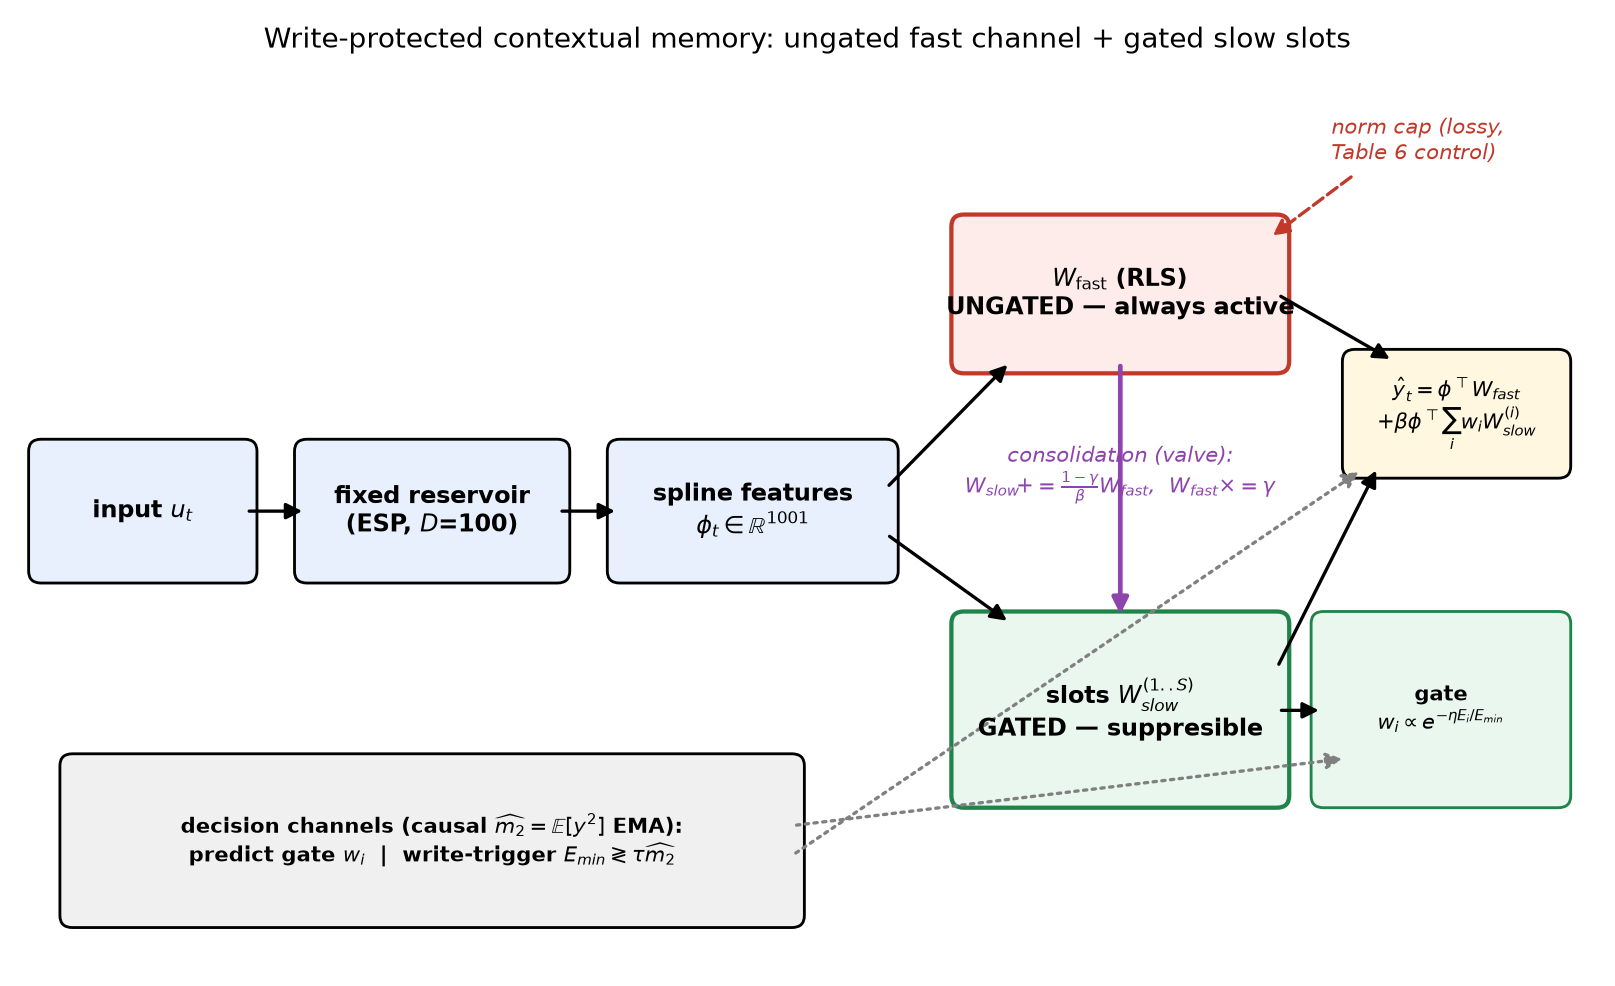
\includegraphics[width=\columnwidth]{fig1_architecture.png}
\caption{Architecture. The ungated fast path $\phi^\top W_{\mathrm{fast}}$ (red) is always active; the gated path $\beta\phi^\top\sum_i w_i W_{\mathrm{slow}}^{(i)}$ (green) is selected by the gate. Consolidation migrates a $(1-\gamma)/\beta$-scaled copy into a slot and decays $W_{\mathrm{fast}}$ by $\gamma$ --- a lossless drainage valve. Two decision channels: prediction gate $w_i$ and write trigger $E_{\min}\lessgtr\tau\hat m_2$. The dashed norm cap is the lossy control of Table~\ref{tab:table6}.}
\label{fig:arch}
\end{figure}

The design targets edge deployment: per-step cost is dominated by
\(O(D K^2)\) floating-point operations (\(\approx 87\) µs readout-only,
\(\approx 130\) µs full system in our Python prototype) and \(O(D K^2)\)
read-write memory (\(\approx 0.13\) MB,
float64), with no gradient
computation, no data storage beyond the current feature vector, and no
GPU requirement.

\subsection{Reservoir and Feature Map}\label{reservoir-and-feature-map}

\textbf{Echo State Network.} The reservoir follows the standard leaky-integrator
update
\[
x_t = (1-\alpha)\,x_{t-1} + \alpha\,\tanh\!\big(W_{\mathrm{res}}x_{t-1} + W_{\mathrm{in}}u_t\big),
\]
with \(D=100\) neurons, input scaling 0.8, leak rate \(\alpha=0.3\), and
10\% sparse connectivity (\(\mathrm{nnz}(W_{\mathrm{res}})=1000\), sampled
without replacement). Rather than relying on the spectral-radius
heuristic, we enforce the sufficient Echo State Property contraction
condition
\[
(1-\alpha) + \alpha\,\|W_{\mathrm{res}}\|_2 < 1
\]
by rescaling \(W_{\mathrm{res}}\) so that \(\|W_{\mathrm{res}}\|_2 = 0.9667\)
(contraction value 0.990). Empirically, five independently initialized
state trajectories converge to pairwise distance \(<10^{-4}\) within
500 steps.
All randomness is drawn from a local generator
(\texttt{np.random.default\_rng(seed)}) so that reported runs are exactly
reproducible.

\textbf{B-spline feature map.} Each reservoir component \(x_t^{(i)}\) is expanded
by \(K=10\) cubic B-spline basis functions over the fixed interval
\([-1,1]\) (the tanh saturation range), yielding \(\phi_t \in
\mathbb{R}^{D\cdot K + 1} = \mathbb{R}^{1001}\) including a bias term.
This additive expansion --- the same construction underlying the recently
proposed Kolmogorov--Arnold-style readouts --- provides the nonlinearity
needed for the linear readout while avoiding the tensor-product blow-up
of multivariate bases. Because each basis is local, the feature vector
is sparse in activation and cheap to evaluate, \(O(D K)\) per step.

\subsection{Block-Diagonal Recursive Least Squares}\label{block-diagonal-recursive-least-squares}

Let \(\phi_t\) be partitioned into \(D\) blocks \(\phi_{t,j} \in
\mathbb{R}^{K}\) plus a scalar bias. Block-Diagonal RLS maintains a
per-block covariance \(P_j \in \mathbb{R}^{K\times K}\) and updates all
blocks through the shared scalar denominator
\[
s_t = \lambda + \sum_{j}\phi_{t,j}^{\top} P_{j}\phi_{t,j} + \phi_{t,b}^{2}P_{b},
\]
followed by per-block Kalman gains \(K_{t,j} = P_{j}\phi_{t,j}/s_t\),
weight update \(W_j \!\leftarrow\! W_j + K_{t,j}e_t\), and covariance
update \(P_j \leftarrow \lambda^{-1}(P_j - K_{t,j}
\phi_{t,j}^{\top}P_{j})\). Formally, this is a full RLS step whose
covariance is projected after each update onto the block-diagonal
subspace: the shared denominator keeps the gains consistent, but the
discarded cross-block terms make the fixed point differ from exact
least squares at finite samples --- the accuracy gap in Table~\ref{tab:table1} is the
price of the projection. Per-step cost drops from \(O(F^{2})\) to
\(O(D K^{2})\) (\(\approx\)\(10^{4}\) vs.~10\(^{6}\) FLOP) and covariance
memory by \(\approx 100\)×. Vectorized via
\texttt{einsum}, the prototype measures \(\approx 87\) µs/update versus
\(\approx 3.8\) ms for full RLS at the \(\lambda{=}0.98\) operating point
--- a \(\approx 44\)× speed-up (the trace bound itself adds
\(\approx 30\) µs/step of trace bookkeeping, a real cost of the
stability mechanism).

\textbf{Covariance windup and trace bounding.} With forgetting factor
\(\lambda<1\) (required for non-stationary tracking), the covariance can
grow exponentially once the signal excites no new directions ---
\emph{covariance windup} --- after which a regime change produces arbitrarily
large weight jumps. We observed precisely this instability in full RLS
at \(\lambda=0.98\) (NMSE diverging beyond 1 within 5000 steps; Fig.~\ref{fig:windup}).
We therefore apply a soft trace bound: whenever
\(\operatorname{tr}(P) > \Pi_{\max}\), rescale \(P \leftarrow
P\,\Pi_{\max}/\operatorname{tr}(P)\), with
\(\Pi_{\max}=10^{4}\,\operatorname{tr}(P_{0})\) --- i.e.
\(10^{4}\!\cdot\!\mathrm{init\_var}\!\cdot\!F\) for full RLS
(\(\approx\!10^{9}\)) and 10\(^{4}\!\cdot\!\mathrm{init\_var}\!\cdot\!K\)
per block for the block engine. Unlike resetting \(P\) to
\(\delta I\), trace scaling preserves the learned anisotropy, and unlike
eigenvalue bounding it costs \(O(K)\) per block. The bound stabilizes
full RLS as well, enabling the ablation in Sec. 4.4 which separates
the structural robustness of the block-diagonal approximation from the
effect of explicit bounding. Two observations temper the picture
(Fig.~\ref{fig:windup}): at \(\lambda{=}0.98\) the bound is engaged
\emph{persistently} rather than as a rare safety valve --- the algorithm
effectively becomes a normalized RLS --- and the unbounded run shows
that divergence is not overflow but the loss of positive-definiteness:
\(\min_j P_{jj}\) first goes negative at \(t{=}1685\), \(\approx 550\) steps
before the prediction error sustains its divergence (\(t{\approx}2234\),
rolling NMSE \(> 10\)× the bounded run).

\subsection{Contextual Memory}\label{contextual-memory}

The memory subsystem is where the contribution of this paper lies; each
of its components exists because a simpler mechanism measurably fails.
We present the final mechanism together with the failure it replaces
(the full empirical ablation is in Sec. 4.4).

\textbf{Architecture.} The readout is split into a fast weight matrix
\(W_{\mathrm{fast}} \in \mathbb{R}^{F\times m}\) trained by RLS every step,
and \(S=3\) slow slots \(W_{\mathrm{slow}}^{(i)}\) that are only written at
consolidation events. Prediction is gated:
\[
\hat{y}_t = \phi_t^{\top}W_{\mathrm{fast}} + \beta\,\phi_t^{\top}\!\Big(\sum_{i=1}^{S} w_i\, W_{\mathrm{slow}}^{(i)}\Big),\qquad
w_i \propto \exp\!\big(-\eta\, E_i / \max(E_{\min},\epsilon)\big),
\]
where \(\eta=2\) sharpens the gate and the \(E_i\) are slow-exponential
context-matching errors (\(\alpha_{\mathrm{ema}}=0.01\)). \(W_{\mathrm{fast}}\)
is trained on the residual target \(y_t - \beta\,\phi_t^\top
\bar{W}_{\mathrm{slow}}\), so the fast component learns only what the
gated slow mixture does not already explain.

\textbf{Failure mode 1 --- unconditional consolidation.} A single slow memory
consolidated unconditionally (every 250 steps,
\(W_{\mathrm{slow}} \mathrel{+}= \tfrac{1-\gamma}{\beta}W_{\mathrm{fast}}\))
does not prevent forgetting: it relocates it. The slow weights become a
lagged copy of the most recent regime, and the return-onset error is
indistinguishable from the memoryless baseline (\naiveOnset{} vs \blockOnset{} NMSE).

\textbf{Failure mode 2 --- self-masking.} With slots introduced, the natural
context-matching error \(e_i = \|y - \phi^\top(W_{\mathrm{fast}} +
\beta W_{\mathrm{slow}}^{(i)})\|^2\) fails, because the fast learner ---
shared by all slots --- compensates for whichever slot currently
contributes, making the active slot appear better than it is. The gate
then locks onto the first consolidated slot and never reallocates. The
fix is to evaluate each slot by what it \emph{alone} explains:
\[
E_i = \|y_t - \beta\,\phi_t^\top W_{\mathrm{slow}}^{(i)}\|^2,
\]
which doubles as an empty-slot detector: an empty slot returns
\(\mathbb{E}[y^{2}]\) (\(=\operatorname{var}(y)\) for the zero-mean targets
in our main protocol; nonzero-mean regimes shift the floor by
\(\mu^{2}\), see Sec. 4.5).

\textbf{Failure mode 3 --- slot poisoning.} With pure \(\arg\min_i E_i\) write
targeting, a slot contaminated by a wrong-regime write can produce
\emph{anti-correlated} predictions whose error exceeds that of an empty slot,
so the minimum hops between slots and writes contaminate good memory
(empirically, a poisoned slot reached \(E_1 = 4.19\) in a diagnostic
run, vs.~\(\widehat{m_2}\approx 0.5\) on the zero-mean stream).
Consolidation therefore requires a gate: write to the
best-matching slot only when it is genuinely matched,
\[
E_{\min} < \tau\,\widehat{m_2},\quad \tau = 0.5
\quad\text{(reinforcement)},
\qquad
\widehat{m_2}\!\leftarrow(1-\alpha_{m_2})\widehat{m_2} + \alpha_{m_2}\|y_t\|^2,
\]
and otherwise write to the emptiest slot (new context) --- never to a
populated high-error slot while an empty slot exists (the saturation
case is treated explicitly below). The signal-energy estimate \(\widehat{m_2}\)
(\(\alpha_{m_2}=0.02\)) is an online running estimate of
\(\mathbb{E}[y^{2}]\) --- \emph{no global or future statistics are used
anywhere in the mechanism}.

\textbf{Failure mode 4 --- norm-based occupancy.} ``Emptiest'' cannot be measured
by \(\|W_{\mathrm{slow}}^{(i)}\|\): regimes produce incomparable weight
magnitudes (square-regime weights had \(\approx 4\)× the norm of sine-regime
weights), so the norm heuristic mistargets writes --- in our runs a
single square-regime consolidation outweighed seven sine consolidations
and contaminated the protected slot (empirically: norm-protected v2
improved 8/10 seeds but degraded 2/10 by up to 20\%, Sec. 4.4). We
instead track
consolidation counts \(c_i\) and select
\(\arg\min_i c_i\), a regime-neutral occupancy measure. This both picks the
right target and cuts variance (std 0.06 → 0.02).

\textbf{Continuity-preserving transfer.} Consolidation into slot \(k\) applies
\[
W_{\mathrm{slow}}^{(k)} \leftarrow W_{\mathrm{slow}}^{(k)} + \tfrac{1-\gamma}{\beta}W_{\mathrm{fast}},
\qquad
W_{\mathrm{fast}} \leftarrow \gamma\,W_{\mathrm{fast}},
\]
with \(\gamma=0.1\). When the gate is confident (\(w_k\approx1\)) the
post-write predictor is algebraically identical to the pre-write one ---
measured discontinuity \(3.4\times10^{-15}\), machine epsilon. For
uncertain gates the jump is bounded by
\((1-w_k)(1-\gamma)\,|\phi^\top W_{\mathrm{fast}}|\). We deliberately do
\emph{not} use the alternative factor \((1-\gamma)/(\beta w_k)\), which enforces
instantaneous continuity at any \(w_k\) but overcharges the slot
(\(\times w_k^{-1}\)) and induces gate oscillation. After each write, the
RLS covariance is inflated by a factor 1.5 to restore fast-memory
plasticity --- a \emph{heuristic} rescaling (modifying weights externally
while keeping the learned covariance anisotropy is not an exact
Bayesian update); alternatives such as full reset or
\(\gamma^{2}\)-scaling were not swept.

\textbf{Write gating during transitions.} Consolidation fires only when the
period counter triggers \emph{and} the fast-error EMA
(\(\alpha_{\mathrm{fast}}=0.1\)) satisfies
\(\bar{e}_{\mathrm{fast}} \le 0.5\,\widehat{m_2}\). During regime
transitions the total error spikes, writes stop, and the gate is given
\(\sim 100\) steps to identify the new context before memory is modified.

\textbf{Saturation policy.} The targeting rule is: if a matched slot
exists, write only to it; otherwise write to the least-consolidated
slot \(\arg\min_i c_i\) --- \emph{including when all slots are populated},
where this becomes consolidation-weighted eviction. Refusing the
write instead (protecting every slot unconditionally) turns out to be
strictly worse, and the reason is structural: consolidation is also
the \textbf{drainage valve} for the fast weights. Blocking it stops the
\(\gamma\)-decay, so \(W_{\mathrm{fast}}\) must absorb the entire
unprotected regime and winds up until it drowns the slow slots'
gated contribution at the next transition (measured: norm \(\approx 30\)
vs \(\approx 2.8\), Sec. 4.6). Eviction, by contrast, is \emph{additive} ---
the displaced slot's content is diluted, not erased --- and the count
rule preferentially sacrifices the least-consolidated context, which
emergently protects long-lived regimes (a desirable side-effect, not
a guarantee: a briefly-seen regime earns few writes and becomes the
eviction candidate). Because fragmentation can consume several slots
per regime (Sec. 4.3), effective capacity counts \emph{allocations}, not
distinct regimes. Overwrite is the default; the main protocol
(2 regimes, 3 slots) never saturates.

\begin{center}\rule{0.5\linewidth}{0.5pt}\end{center}

\section{Experiments}\label{experiments}

\subsection{Setup}\label{setup}

\textbf{Tasks.} (i) \emph{Sine→Square→Sine}: three phases of 1500 steps each,
input \(u_t\) and target \(u_{t+1}\) from the indicated waveform (period 80);
the primary forgetting-cost benchmark. (ii) \emph{MG-17→MG-30→MG-17}:
Mackey--Glass prediction (\(\dot{x} = \beta x_\tau/(1+x_\tau^{10}) - \gamma x\),
\(\beta{=}0.2,\gamma{=}0.1\)) switching between delays \(\tau{=}17\) and
\(\tau{=}30\); similar-dynamics control. (iii) \emph{NARMA-10→MG-17→NARMA-10}:
the driven memory task \(y_{t+1} = 0.3y_t + 0.05y_t\sum_{i=0}^{9}y_{t-i}
+ 1.5u_{t-9}u_t + 0.1\), \(u\sim U[0,0.5]\), interleaved with the chaotic
task; dissimilar-dynamics test. All runs use 500-step washout, reservoir
\(D{=}100\), features \(D K{+}1\), \(\lambda{=}0.98\), \(\mathrm{init\_var}
{=}10^{2}\), trace bound \(\Pi_{\max}=10^{4}\cdot\operatorname{tr}(P_0)\)
(Sec. 3.3).

\textbf{Metrics.} Per-phase onset NMSE (first 250 steps; sensitivity to the
window length is reported in Sec. 4.4) and end NMSE (last 250 steps),
normalized by the \emph{global} target variance --- used only for
\emph{evaluation}, never as a mechanism input; all mechanism thresholds use
the online estimate \(\widehat{m_2}\) of Sec. 3.4. Input streams are
standardized globally as a benchmark design constant (in deployment
this would be a fixed sensor-scale constant or a slow online estimate;
noted as a limitation). Wall-clock timings were measured on an Intel
Family-6 Model-141 CPU, Python 3.13.14, NumPy 2.5.2/OpenBLAS 0.3.34,
single process. Output dimension \(m=1\) throughout; \(W_{\mathrm{in}}
\in\mathbb{R}^{D\times1}\) with input scaling 0.8. Empirical ESP was
accepted at pairwise state distance \(<10^{-4}\) after 500 steps.
Baselines: batch ridge, full RLS, block-diagonal RLS, naive dual
memory, competitive multi-head readout (Bereska-style), and staged
contextual-memory ablations.

\subsection{Readout Characterization}\label{readout-characterization}

Table~\ref{tab:table1} summarizes the Mackey--Glass study. Block-diagonal RLS
trades an order of magnitude of asymptotic accuracy for
\(\approx 44\)× update speed and \(\approx 100\)× covariance memory
versus full RLS at the \(\lambda{=}0.98\) operating point ---
the regime relevant to edge deployment.

\begin{table}[t]
\centering\small
\caption{Readout characterization on MG-17 ($D{=}100$, $K{=}10$,
$F{=}1001$). $\lambda{=}1$ NMSEs are representative values from the
10-seed characterization; $\lambda{=}0.98$ rows are single-seed
diagnostics at the operating point used throughout. Accuracy gap
$\approx14\times$, speed gap $\approx44\times$ at that point --- the
faster 53 \textmu s/step figure at $\lambda{=}1$ is \emph{not} the
configuration used in this paper (the bound adds $\approx 30$
\textmu s).}
\label{tab:table1}
\begin{tabular}{lcccc}
\toprule
Method & $\lambda$ & NMSE @5000 & Update & $P$ memory \\
\midrule
Ridge (batch) & --- & $\approx$9e-6 & offline & --- \\
Full RLS & 1.0 & $\approx$1e-3 & 3.4 ms/step & 7.6 MB \\
Block-RLS & 1.0 & $\approx$2e-2 & 53 \textmu s/step & 78 kB \\
Full RLS + bound & 0.98 & 8.1e-3 & 3.8 ms/step & 7.6 MB \\
Block-RLS + bound & 0.98 & 0.115 & 87 \textmu s/step & 78 kB \\
\bottomrule
\end{tabular}
\end{table}

At \(\lambda=0.98\) unbounded full RLS diverges by
covariance windup while the trace bound restores stability in both
engines (Fig.~\ref{fig:windup}). The bound removes a confound for Sec. 4.3: with
bounding, full RLS still degrades badly at regime return (onset NMSE
\(8.17\pm4.0\), median 6.9, IQR {[}4.6, 10.9{]}, vs 0.46\(\pm0.22\) for block
RLS) --- suggesting, though not proving, that the block-diagonal
approximation is structurally more robust under regime reversal, since
over-specialized cross-block correlations hurt precisely when the
readout must revert.

\subsection{Main Protocol: Sine→Square→Sine}\label{main-protocol-sinesquaresine}

\begin{figure}[t]
\centering
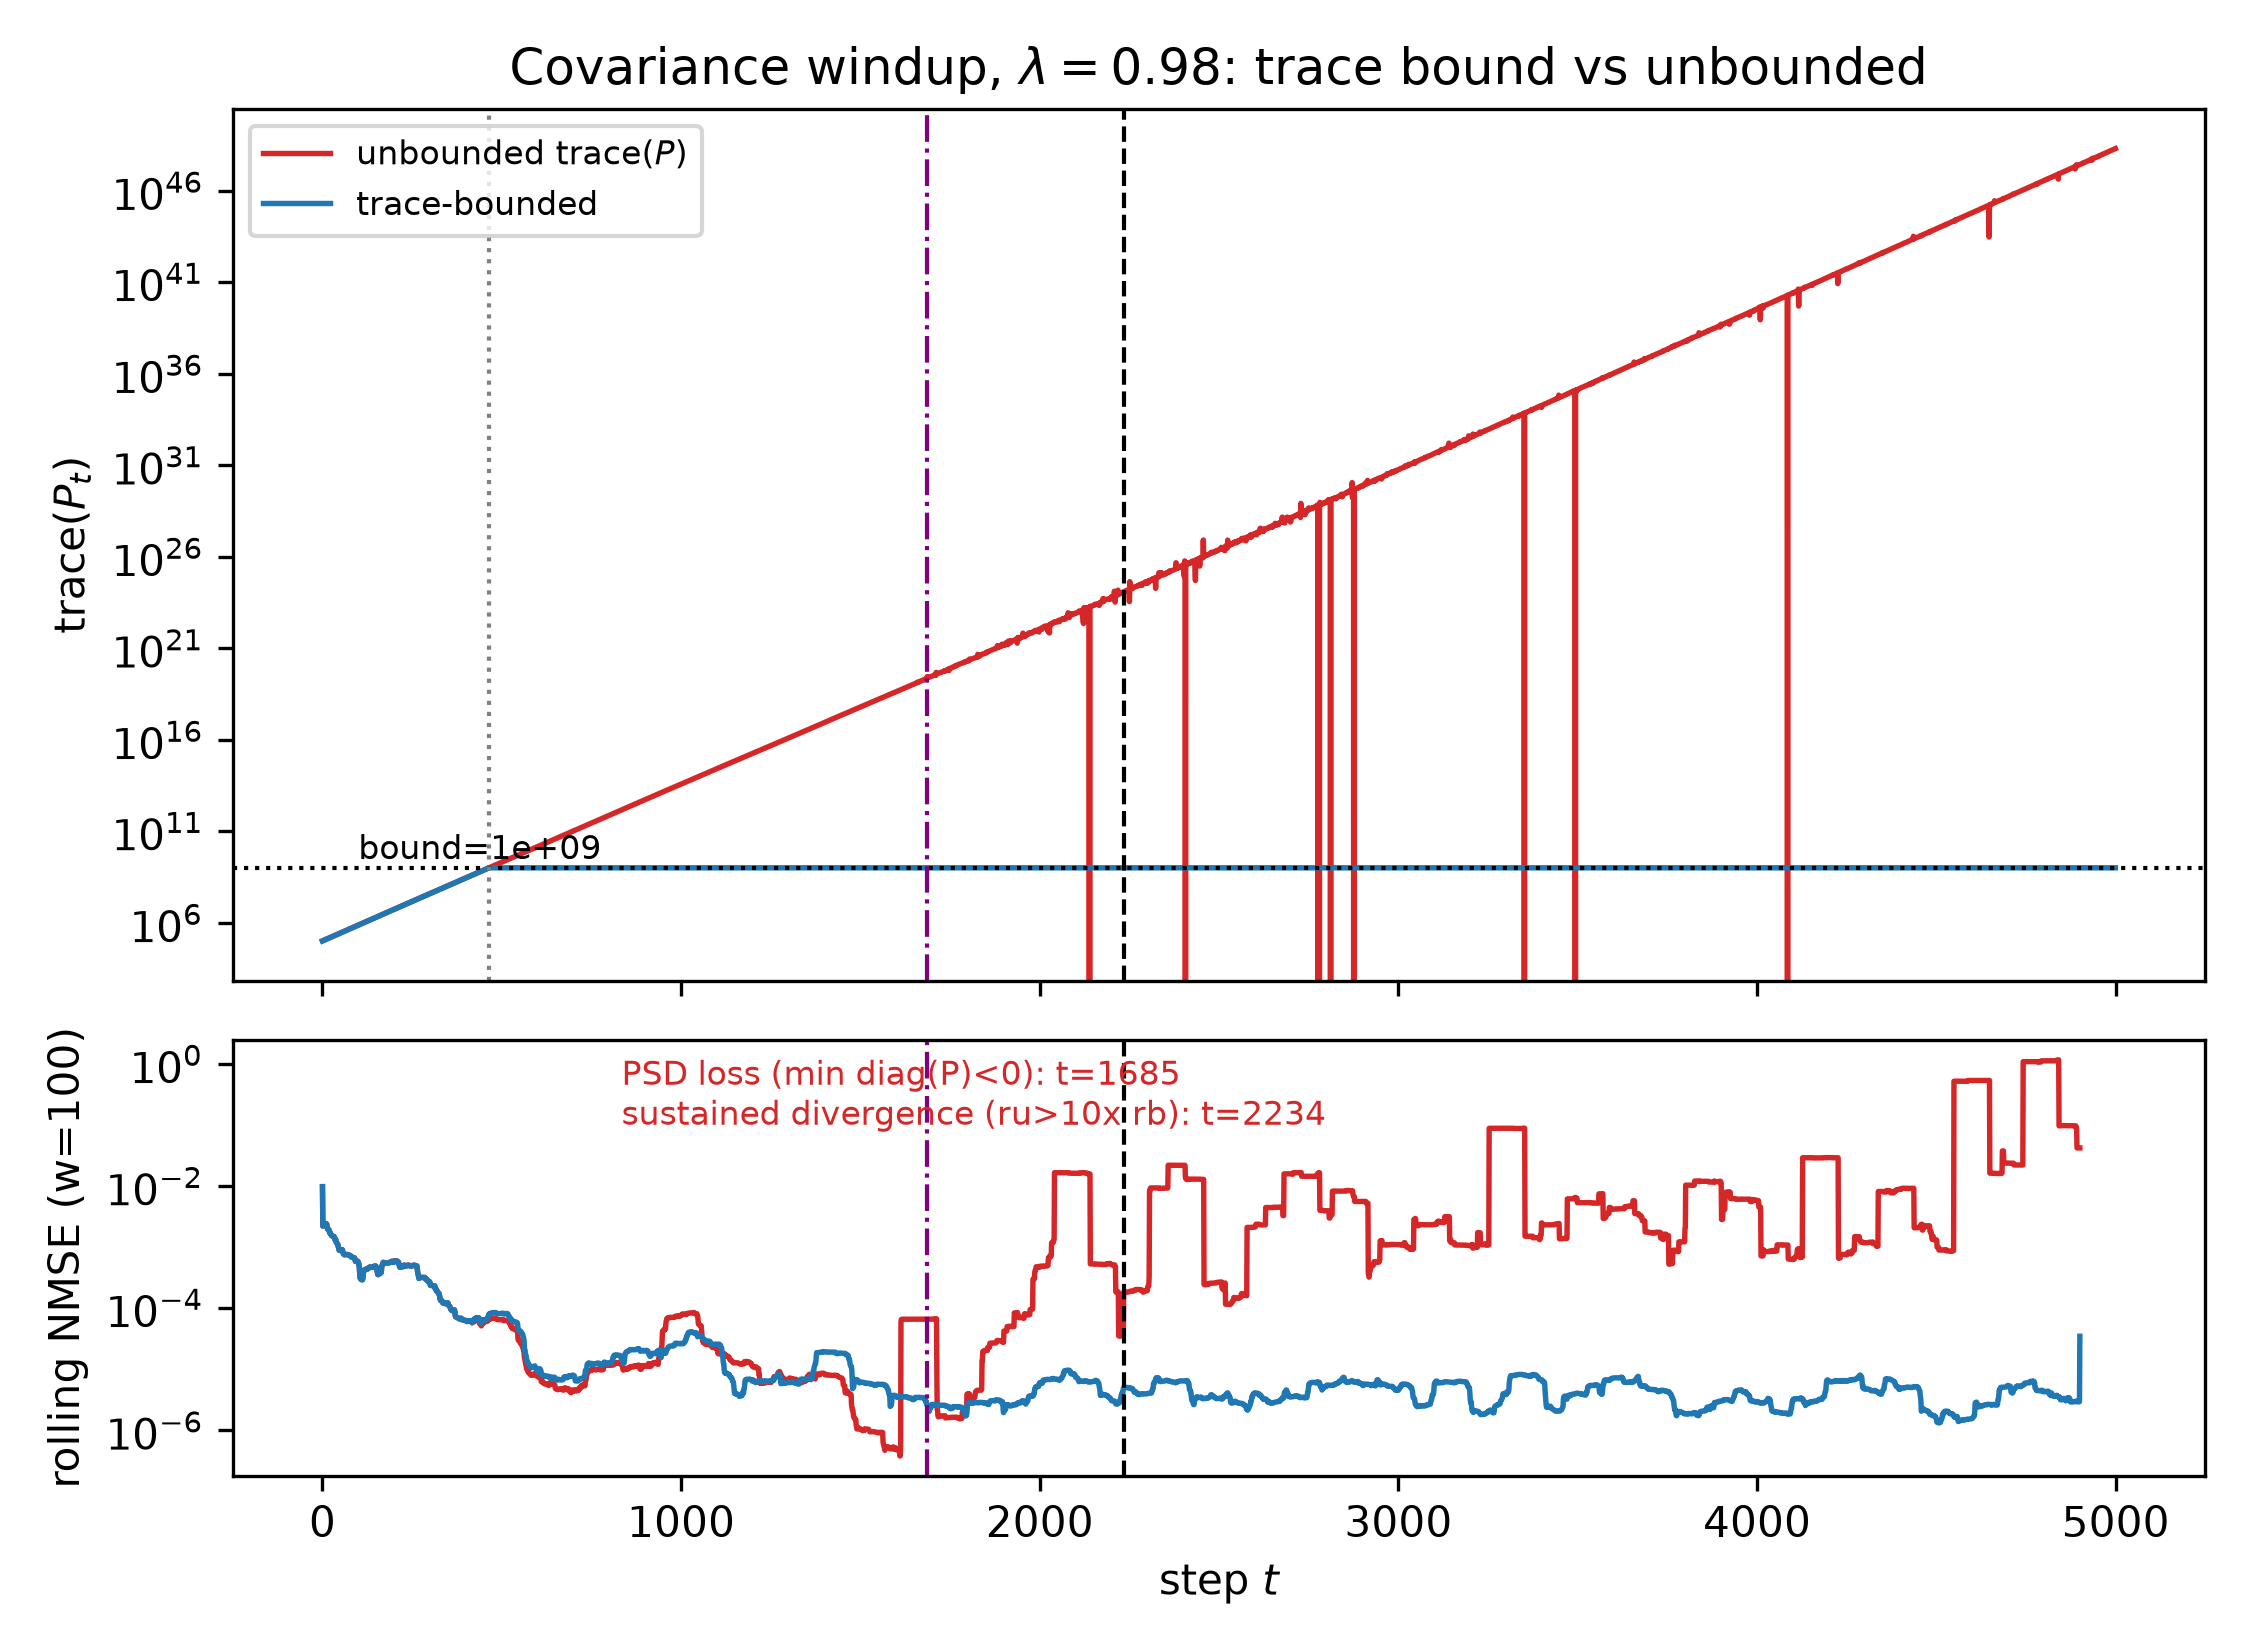
\includegraphics[width=\columnwidth]{fig2_windup.png}
\caption{Covariance windup at $\lambda{=}0.98$ (representative seed). Top: unbounded $\mathrm{tr}(P)$ reaches $\sim10^{48}$; the trace bound $\Pi_{\max}{=}10^4\mathrm{tr}(P_0)$ is a chosen reference, persistently active --- the effective algorithm approaches normalized RLS. Bottom: rolling NMSE. The chain: bound crossing ($t{\approx}465$) $\to$ first $\min\mathrm{diag}(P){<}0$ ($t{=}1685$) $\to$ sustained divergence ($t{=}2234$, rolling NMSE $>10\times$ bounded run). Divergence is loss of positive-definiteness, not overflow.}
\label{fig:windup}
\end{figure}

\begin{table}[t]
\centering\small
\caption{Regime-return protocol
(sine$\to$square$\to$sine), 10 seeds, mean$\pm$std where variable.
F3-onset = NMSE over the first 250 steps of the sine return;
normalization uses the global target variance as a constant
evaluation scale (Sec. 4.1).}
\label{tab:table2}
\begin{tabular}{lcccc}
\toprule
Method & F1-end & F2-end & F3-onset (primary) & F3-end \\
\midrule
FullRLS+bound & 3.8e-11 & 0.108 & $8.17\pm3.92$ & 2.3e-05 \\
BlockRLS+bound & 1.6e-04 & 0.545 & $0.459\pm0.22$ & 1.0e-02 \\
+naive memory & 1.6e-04 & 0.543 & 0.455 & 1.0e-02 \\
+MultiHead (prior art) & 1.6e-04 & 0.545 & $0.424\pm0.17$ & 9.3e-03 \\
+MultiHead+alloc & 1.6e-04 & 0.548 & $0.377\pm0.14$ & 7.6e-03 \\
+MultiHead+alloc+soft & 1.6e-04 & 0.548 & $0.291\pm0.10$ & 7.6e-03 \\
\textbf{+CTX (final)} & 1.9e-04 & 0.460 & $\mathbf{0.104\pm0.02}$ & 3.7e-02 \\
\bottomrule
\end{tabular}
\end{table}

Table~\ref{tab:table2} reports 10 seeds. The contextual memory reduces return-onset
NMSE from \(\blockOnset\pm0.22\) to 0.104\(\pm0.02\) --- a \textbf{4.40× improvement,
positive in 10/10 seeds} (range 0.067--0.128 vs.~baseline 0.18--0.91;
worst case 0.913→0.081). The gain is not an artifact of the window
definition: at onset windows 100/250/500 the improvements are
×4.41/×4.40/×4.66. The closest prior approach --- three competitive
RLS heads selected by EMA error (Bereska-style passive protection) ---
achieves only \mhOnset{} and is \emph{bit-identical} to the memoryless baseline
in 9/10 seeds --- its protection mechanism never engages; in the single
seed where the gate fires it does work (0.913→0.546), which is the
conditional claim we make about it. The mechanism-level reason is
instructive: its only differentiation channel is the prediction gate,
and an \emph{empty} head returns the signal-energy floor
\(\mathbb{E}[y^2]\approx1\), which the sine-trained head's
\(\approx 0.7\) cross-regime error on the partially correlated square
wave never exceeds --- so the gate never reallocates and the passive
protection never engages. Our write-protection rule supplies the
missing second channel: even while the gate remains on slot 0 during
phase 2, \(E_{\min}>\tau\widehat{m_2}\) routes writes to new slots.
To isolate this channel we augmented the competitor with
write-triggered allocation (\emph{MultiHead+alloc}: a never-updated head
is selected when \(E_{\min}>\tau\widehat{m_2}\), same \(\tau\)): it
recovers part of the gap (\(0.424\to0.377\), improving substantially
the seeds where the gate floor had blocked allocation --- 1, 6, 8 ---
and marginally seed 7).
Next we port the normalized soft gate itself (relative errors
\(E_i/\max(E_{\min},\epsilon)\), \(\eta{=}2\), mixture prediction with
winner-only updates): \emph{MultiHead+alloc+soft} reaches \(0.291\),
i.e.~the two borrowed components account for
\(0.424\to0.291\approx\times1.5\) of the competitor's gap. The
remaining \(\approx 2.8\)× to CTX cannot come from gating --- the
competitor has no ungated channel to manage --- and is therefore
attributable to the dual-rate transfer architecture itself
(damped fast weights plus continuity-preserving consolidation).
Decomposition caveat: these two interventions are not orthogonal
(soft gating alone yields 0.323), so we report the laddered
rather than a factorial attribution. Note the trigger is not free:
early allocation slightly degraded two seeds
(2: \(0.312\to0.314\), +0.8\%; 9: 0.385\(\to0.408\), +6.1\%). A Wilcoxon signed-rank test confirms
significance (one-sided Wilcoxon signed-rank, \(W{=}55\),
\(p{=}9.8\times10^{-4}\); paired \(t_{9}{=}4.71\), \(p{=}1.1\times10^{-3}\);
the prespecified primary endpoint is phase-3 onset NMSE at the 250-step
window). The naive dual memory is
statistically indistinguishable from baseline (\naiveOnset), confirming that
consolidation \emph{per se} contributes nothing --- protection and targeting do.

Fig.~\ref{fig:traj} (seed 0) shows the mechanism: at the square→sine boundary
(\(t{=}3000\)) the contextual system falls below NMSE 0.1 within
\(\approx 250\) steps while the baseline requires \(\gtrsim 1000\) steps to
reach the same level. Fig.~\ref{fig:gate} visualizes the gate: slot 0 captures
phase 1 (\(w_0\!\approx\!1\)); in phase 2 slots 1--2 share the gate with a
periodic modulation (the square wave \(\approx\operatorname{sign}(\sin)\)
partially matches the sine slot each half-cycle --- visible as vertical
banding); in phase 3 the gate returns to slot 0 within the EMA
timescale and stays there. The two-slot phase-2 allocation has a
mechanistic explanation confirmed by consolidation logs: the square
regime is intrinsically harder for this reservoir (end NMSE
\(\approx0.46\)), so \emph{no} slot's slow-only error falls below
\(\tau\,\widehat{m_2}\) --- every write is treated as new context and the
count rule round-robins slots 1\(\leftrightarrow 2\). This exposes a
predictability--novelty conflation: the threshold cannot distinguish
``new regime'' from ``current regime is hard''. We return to this in
Sec. 5.

\begin{figure}[t]
\centering
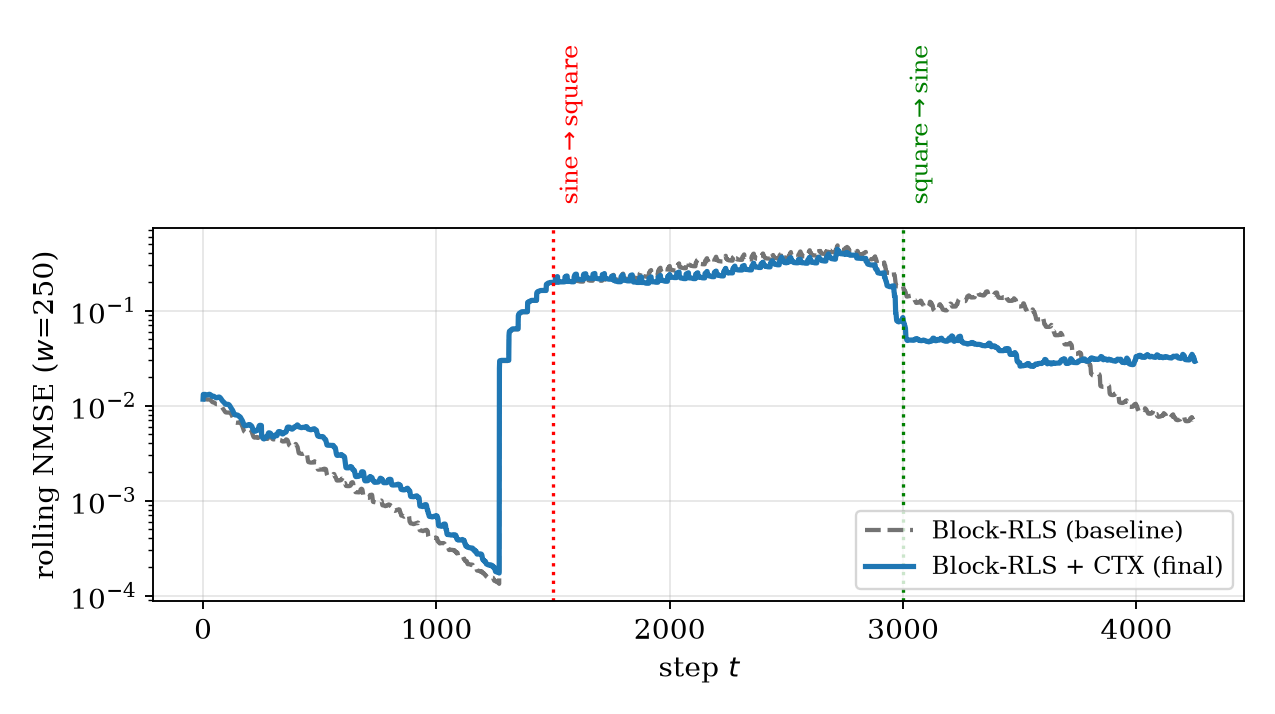
\includegraphics[width=\columnwidth]{fig3_error_trajectory.png}
\caption{Regime return, seed 0: rolling NMSE ($w{=}250$, normalized by $\sigma_0$). At the square$\to$sine boundary CTX re-engages the stored sine slot while the memoryless baseline re-learns from scratch.}
\label{fig:traj}
\end{figure}

\begin{figure}[t]
\centering
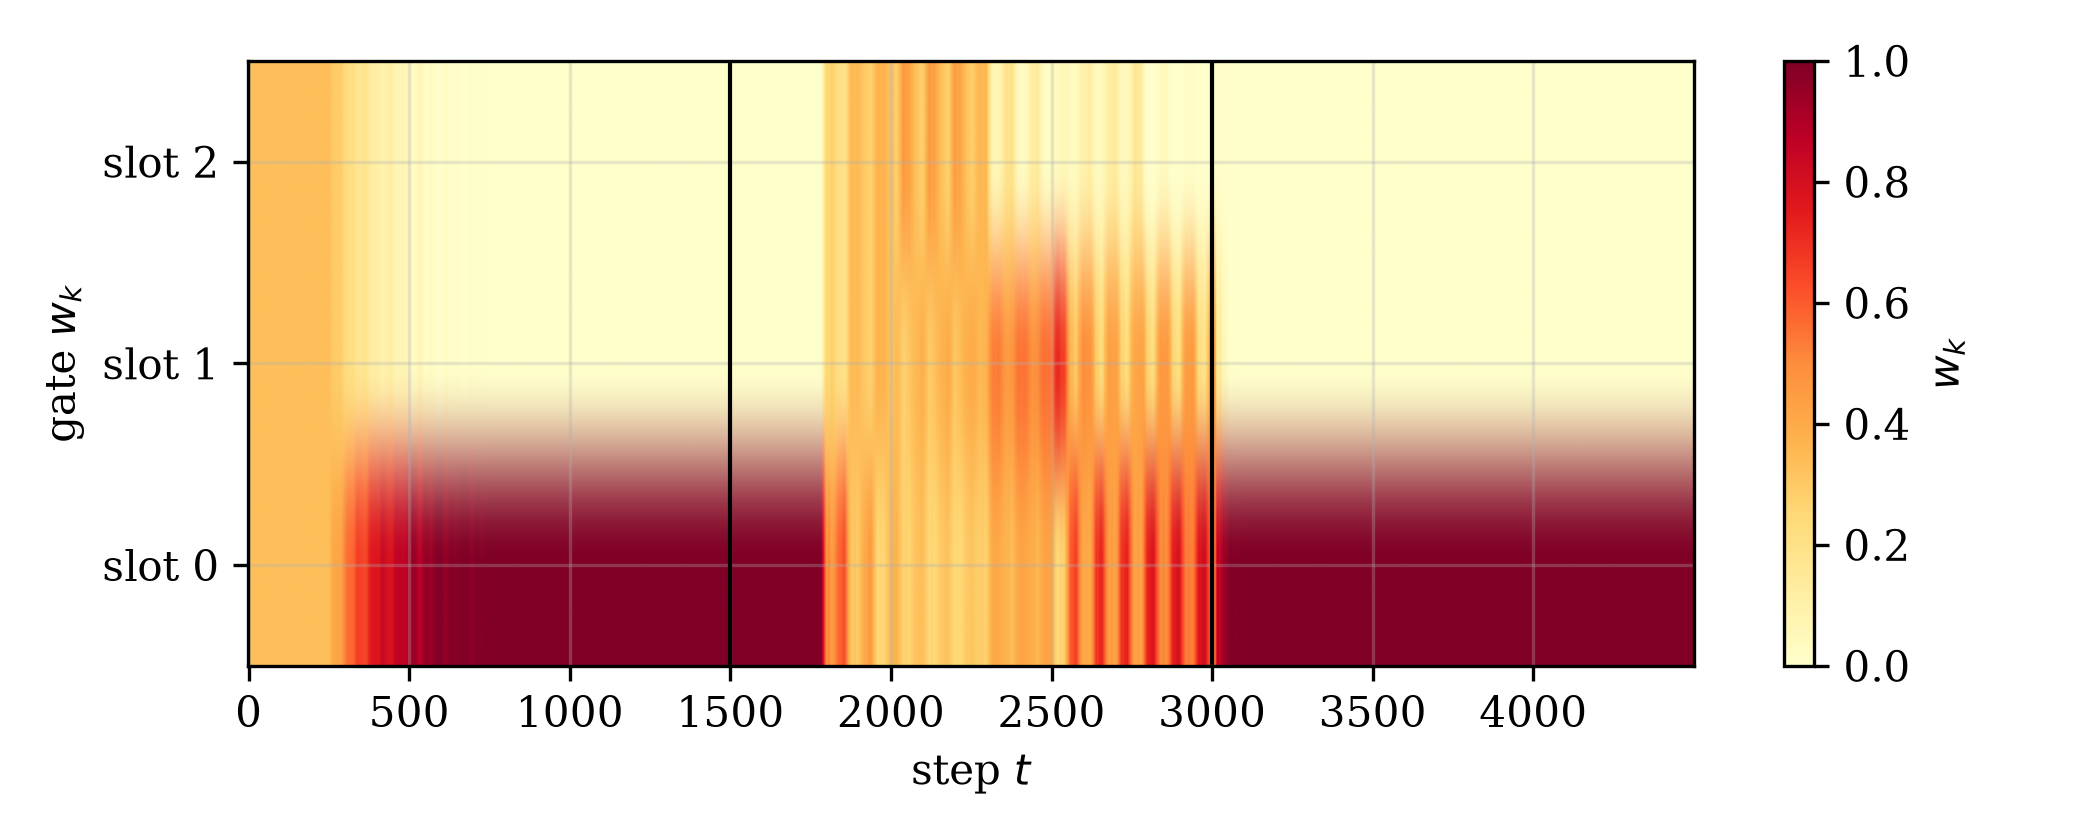
\includegraphics[width=\columnwidth]{fig4_slot_heatmap.png}
\caption{Gate weights $w_k$ across the protocol (seed 0). Slot 0 captures the sine regime; the square phase fragments writes across slots 1--2 (novelty/unpredictability conflation, Sec. 5). At the sine return the gate selects the correct slot.}
\label{fig:gate}
\end{figure}

Consolidation logs confirm the mechanism end-to-end for seed 0: phase-1
writes reinforce slot 0 (\(E_0\to0.003\)); phase-2 writes alternate
between slots 1--2 as new context while slot 0's error stays
\(E_0\!\approx\!1.5\) --- contaminated but \emph{unwritten}; phase-3 writes
return to slot 0 once \(E_0\) falls below \(\tau\,\widehat{m_2}\).

\textbf{Costs.} End-of-phase accuracy is \ctxEndPenalty\(\times\) worse under CTX
(\(3.7\!\times\!10^{-2}\) vs 1.0\(\!\times\!10^{-2}\)), attributable to the
\(\gamma{=}0.1\) fast-weight decay at each write slowing final
convergence, and the bounded transition jump (max 1.49 instantaneous
prediction change, measured at write instants on the current feature
vector) is confined to bootstrap writes at uniform gates.

\subsection{Ablation Study}\label{ablation-study}

Tables~\ref{tab:table3a}--\ref{tab:table3b} and Fig.~\ref{fig:ablation} isolate each mechanism on 10 seeds. Table~\ref{tab:table3a}
shows the \emph{cumulative} CTX ablation ladder --- each layer repairs a
documented failure mode --- while Table~\ref{tab:table3b} is the separate
\emph{competitor ladder} used for attribution (Sec. 4.3):

\begin{figure}[t]
\centering
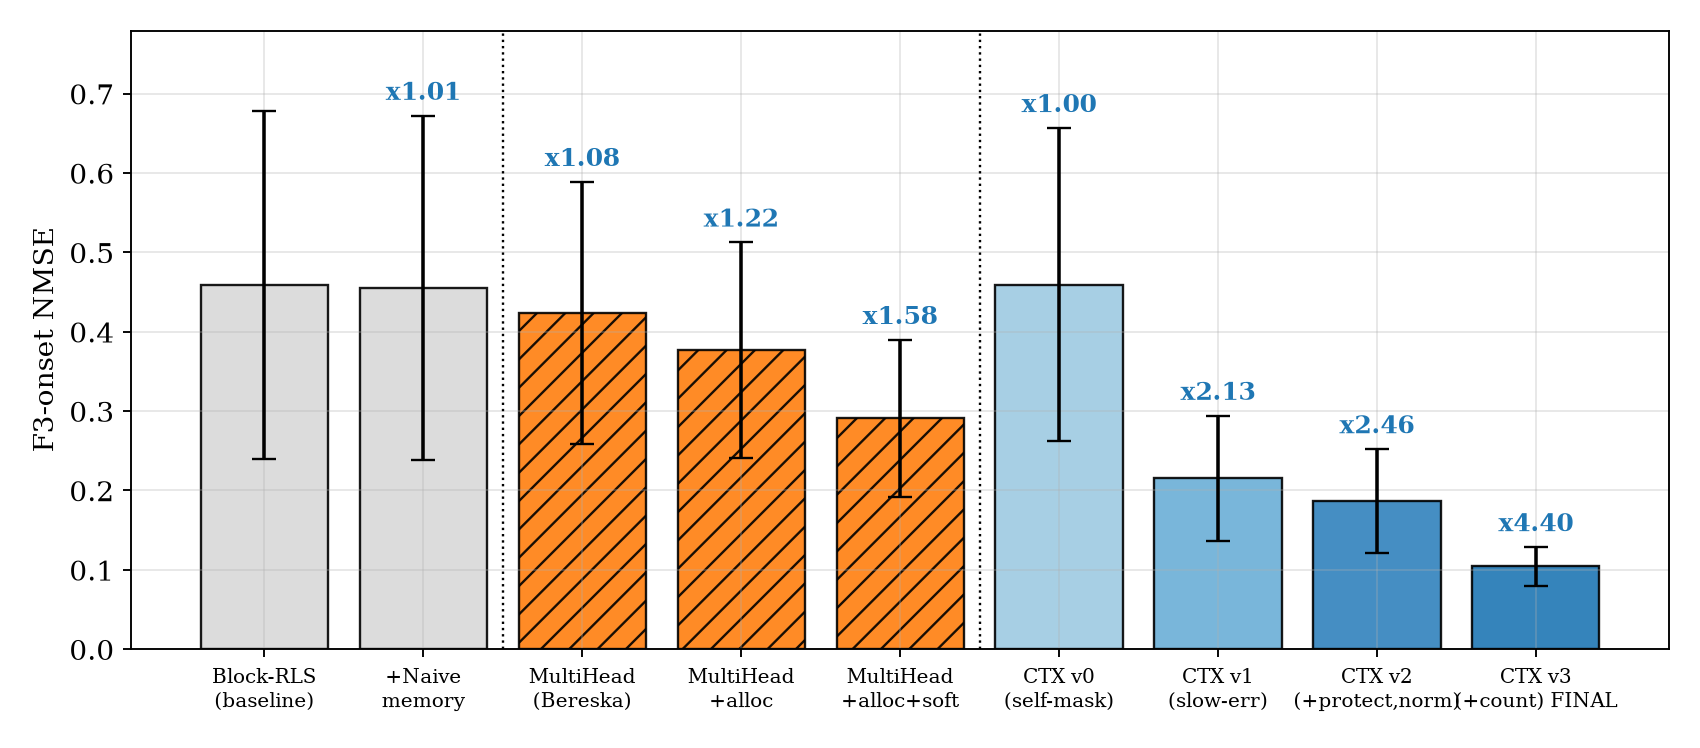
\includegraphics[width=\columnwidth]{fig5_ablation_bar.png}
\caption{Ablation and competitor ladder, 10 seeds (mean$\pm$std). Three families: baselines (grey), competitor ladder (orange, hatched), CTX ladder (blue). Annotations give the ratio against the memoryless baseline.}
\label{fig:ablation}
\end{figure}

\begin{table}[t]
\centering\small
\caption{Cumulative ablation of the proposed mechanism, 10 seeds.}
\label{tab:table3a}
\begin{tabular}{lcl}
\toprule
CTX layer & F3-onset NMSE & Interpretation \\
\midrule
Block-RLS & $0.459\pm0.22$ & baseline \\
+naive memory & 0.455 & consolidation relocates forgetting \\
+CTX v0 (self-masked) & 0.455 & reproduced defect: shared $W_{\mathrm{fast}}$ masks slot quality \\
+CTX v1 (slow-error) & $0.204\pm0.07$ & unmasking halves onset error \\
+CTX v2 (+protection, norm) & $0.183\pm0.06$ & mean gain n.s.\ ($p{=}0.116$); regressions in 3/10 seeds \\
+CTX v3 (+cons.\ count) & $\mathbf{0.096\pm0.02}$ & correct target \emph{and} low variance \\
\bottomrule
\end{tabular}
\end{table}

\begin{table}[t]
\centering\small
\caption{Bereska-style competitor strengthened with our components
(laddered, not factorial); the residual gap is architectural.}
\label{tab:table3b}
\begin{tabular}{lcl}
\toprule
Competitor ladder & F3-onset NMSE & Interpretation \\
\midrule
MultiHead (prior art) & $0.422\pm0.16$ & passive protection never engages \\
MultiHead+alloc & $0.369\pm0.13$ & write-trigger channel: helps seeds 1, 6, 8 \\
MultiHead+alloc+soft & $0.268\pm0.09$ & +normalized gate: borrows $\times1.6$ of gap \\
CTX (ours) & $\mathbf{0.096\pm0.02}$ & remaining $\approx$2.8$\times$ = dual-rate transfer \\
\bottomrule
\end{tabular}
\end{table}

The v1→v2 comparison carries the subtle finding: the norm proxy's
average gain is \emph{not significant} (one-sided Wilcoxon \(W{=}43\),
\(p{=}0.065\)) and comes with targeted regressions --- 8/10 seeds
improved, yet seeds 0 and 5 degraded (worst: seed 0,
0.147→0.176, +20\%; seed 5: 0.258→0.303, +18\%)
because a wrongly chosen slot is \emph{preserved} rather than overwritten.
In other words, a bad oracle turns protection into a \emph{gamble}; a
correct oracle turns it into a \emph{guarantee}: occupancy counts beat the
norm variant in 10/10 seeds (Wilcoxon \(p{<}10^{-3}\)), improve the mean
(0.187→0.104), and cut dispersion threefold (std 0.07→0.02). The
statistical picture is consistent with that reading: the two
mechanism repairs are each individually significant (v0→v1 and
v2→v3, both \(p{<}10^{-3}\) and surviving a Holm correction across the
four comparisons), while the norm-proxy step is the only
nonsignificant one --- the gain lives in reliability, not in the mean,
because protection is only as good as the emptiness oracle it
consults.

\subsection{Generalization Across Dynamics}\label{generalization-across-dynamics}

\begin{table}[t]
\centering\small
\caption{F3-onset NMSE on cross-family dynamics; MultiHead equals the
baseline to printed precision.}
\label{tab:table4}
\begin{tabular}{lccccc}
\toprule
Protocol (5 seeds) & Block & MultiHead & CTX & Gain & Slots \\
\midrule
MG-17$\to$MG-30$\to$MG-17 & 1.40e-2 & 1.40e-2 & 1.38e-2 & $\times$1.01 & [0,0,0] 5/5 \\
NARMA-10$\to$MG-17$\to$NARMA-10 & 0.108 & 0.108 & 0.104 & $\times$1.04 & [0,1,0] 3/5 \\
\bottomrule
\end{tabular}
\end{table}

Table~\ref{tab:table4} tests whether the mechanism generalizes beyond the benchmark it
was tuned on. On NARMA-10→MG-17→NARMA-10 the slots discriminate
correctly ({[}0,1,0{]} in 3/5 seeds) yet the gain is modest (×1.05) because
NARMA-10 is cheap to relearn on this reservoir --- baseline onset already
nearly equals end error (0.108 vs 0.106), leaving little margin to
recover; the \(\mu^2\) term in \(\widehat{m_2}\) also weakens context
discrimination for nonzero-mean targets (5/5 clean patterns under a
variance oracle). On MG-17→MG-30→MG-17 the gain is \(\approx\times 1.01\) with all
writes reinforcing slot 0: the two delays produce readouts similar
enough that slot errors never separate, no context is ever written, and
the mechanism passivates \emph{harmlessly}. The multi-head baseline reduces
to the memoryless baseline on both tasks for the same empty-floor
reason as in Sec. 4.3.

Together with the main protocol, the three tasks establish a
\textbf{cost-proportional benefit} property: the memory pays nothing when
there is nothing to protect, and gains most where forgetting is
expensive (sine\(\leftrightarrow\)square: ×4.40). The worst observed regression for
the \emph{final} mechanism across all experiments is one NARMA seed at 14\%
(intermediate ablation variants reach +20\%; the refuse saturation
policy costs +6\% --- harmlessness holds while drainage is active and
slot demand fits capacity, see Sec. 4.6).

\subsection{Saturation Policy Under Overload}\label{saturation-policy-under-overload}

The ``never write to a populated slot'' invariant is only defined while
an empty slot exists. We stress it with a four-regime protocol
(sine→square→triangle→sine) in which slot demand exceeds supply: with
\(S{=}2\) the square and triangle phases both request new-context
writes against a fully populated memory, and with \(S{=}3\)
fragmentation (Sec. 4.3) can still exhaust the budget. Table~\ref{tab:table5}
compares the two policies of Sec. 3.4 on the phase-4 sine return.

\begin{table}[t]
\centering\small
\caption{Saturation mini-ablation, 10 seeds ($S{=}2$ grid plus
$S{=}3$). Clamp $R{=}3.18$ = median $\|W_{\mathrm{fast}}\|$ over the
overwrite run after phase 1, calibrated on seed 0 --- a single-seed
trajectory median, acceptable here because refuse norms are an order
of magnitude larger, so the comparison is insensitive to the exact
radius. Refuse collapses to baseline; a bare norm clamp restores
recall almost completely.}
\label{tab:table5}
\begin{tabular}{lcc}
\toprule
Configuration & F4-onset NMSE & $\|W_{\mathrm{fast}}\|$ at boundary \\
\midrule
Block-RLS (memoryless) & $0.069\pm0.024$ & 34.7 \\
Block-RLS + clamp & $0.051\pm0.014$ & 3.2 \\
$S{=}2$, refuse & $0.074\pm0.031$ & 36.1 \\
$S{=}2$, refuse + clamp & $0.019\pm0.013$ & 3.2 \\
$S{=}2$, overwrite & $\mathbf{0.016\pm0.002}$ & 0.31 \\
$S{=}3$, overwrite & $0.023\pm0.012$ & --- \\
$S{=}3$, refuse & $0.072\pm0.028$ & --- \\
\bottomrule
\end{tabular}
\end{table}

The outcome is the opposite of the naive intuition that refusing
writes is the safer protection, and it opens an obvious confound ---
\emph{is the benefit memory or merely regularization?} A full factorial
answers it. Under \emph{refuse} every write after step 2000 is skipped, so
the \(\gamma\)-decay that damps \(W_{\mathrm{fast}}\) after each
consolidation never fires: the fast weights absorb the entire
unprotected regime and wind up to \(\|W_{\mathrm{fast}}\|\approx35\)
(Fig.~\ref{fig:valve}). At the sine return the gate \emph{does} select the correct slot,
but the giant stale fast contribution drowns its output. Two
measurements isolate the cause. (i) \emph{Correlation}: pooled across all
configurations and seeds, \(\log\|W_{\mathrm{fast}}\|\) at the
phase-4 boundary predicts onset error (Spearman \(\rho{=}0.82\),
\(p{=}1.5\times10^{-10}\), \(n{=}40\)) --- mostly a between-condition
separation, though a marginal trend survives within refuse alone
(\(\rho{=}0.60\), \(p{=}0.067\), \(n{=}10\), underpowered).
(ii) \emph{Intervention}: clamping
\(\|W_{\mathrm{fast}}\|\) under refuse --- touching nothing else ---
restores recall to \(0.019\approx 0.016\) (overwrite-level). The stored
memory was intact all along; it was simply unreachable beneath the
bloated fast weights. Yet drainage alone is not the whole story:
clamping the \emph{memoryless} baseline helps only marginally
(\(0.069\to0.051\)), so the slot content contributes a further
\(\approx 2.7\)× --- memory provides the material, drainage provides
access to it, and the naive variant already proves drainage without
separable memory is worthless on the main protocol. Caveat: this
four-regime stream is a \emph{cheap-relearning} regime (baseline onset
0.069 vs 0.46 on the main protocol; per-phase end NMSEs
{[}0.000, 0.34, 0.18, 0.003{]}), so the absolute gains here measure the
drainage mechanism, not memory value at scale.

We therefore repeat the decisive control on the main protocol itself
(Table~\ref{tab:table6}). The clamp radius is now protocol-specific:
\(R{=}0.94\), the median \(\|W_{\mathrm{fast}}\|\) observed at the full
mechanism's own consolidation events (180 events pooled over the same
10 seeds) --- a matched-norm control that is not tuned on the test
metric. On sine→square→sine, clamping a memoryless baseline recovers
part of the headline gain (\blockOnset→\clampOnlyOnset, \(\times2.07\),
\(p{=}0.003\)), but the stored context still contributes a further
\(\times2.13\) (\clampOnlyOnset→0.104, \(p{=}0.001\)). So the \(\times4.40\)
improvement factors into roughly equal components: fast-channel
drainage (\(\times2.07\)) and gated slot content (\(\times2.13\)). Like
the competitor ladder above, this is a \emph{laddered} (order-dependent)
decomposition: the second step both removes the lossy cap and adds
slots plus lossless transfer, so \(\times2.13\) is an upper bound on
the memory component alone.

Crucially, the two drainage styles are not equivalent. A hard norm
cap buys onset at the price of \emph{end-phase} accuracy: the clamped
weights cannot regrow to re-fit the returned regime, so its F3-end
error degrades to \clampEnd{} --- \(\approx 40\)× worse than the uncapped
baseline and \(\approx 11\)× worse than CTX. The transfer mechanism achieves the same drainage
losslessly, by moving the information into the gated channel rather
than destroying it: CTX pays only the mild \(\gamma\)-decay cost
(\(\blockEnd\to\ctxEnd\)). This is the measured answer to ``why not just cap
the norm?'': a cap is a lossy valve, consolidation is a lossless one.

\begin{table}[t]
\centering\small
\caption{Drainage control on the main protocol, 10 seeds. The norm
cap alone recovers $\times 2.07$; gated memory a further $\times 2.13$;
but the lossy cap destroys end-phase accuracy while transfer does
not.}
\label{tab:table6}
\begin{tabular}{lcc}
\toprule
Configuration & F3-onset NMSE & F3-end NMSE \\
\midrule
Block-RLS & $0.459\pm0.219$ & 0.010 \\
Block-RLS + clamp ($R{=}0.94$) & $0.222\pm0.010$ & 0.405 \\
CTX (full) & $\mathbf{0.096\pm0.021}$ & 0.037 \\
\bottomrule
\end{tabular}
\end{table}

The lesson generalizes: \textbf{the consolidation channel is also a
pressure-release valve for the fast weights} --- refuse protects
memory \emph{content} but starves the valve, converting stored memory into
memory that exists yet cannot be reached in time. Under \emph{overwrite},
two properties combine favorably: the count rule evicts the
least-consolidated slot (slot 0's 13 writes make it nearly
eviction-proof), and eviction is \emph{additive} --- content is diluted, not
erased. Where all stored contexts must outrank the current one, a
norm cap on \(W_{\mathrm{fast}}\) is mandatory whenever writes are
refused. A residual trade is visible in Fig.~\ref{fig:valve}'s end phase: refuse,
which never drains, avoids the \(\gamma\)-decay cost that overwrite
pays at every consolidation --- it loses the onset but wins the tail.

\subsection{Cost Profile}\label{cost-profile}

\begin{figure}[t]
\centering
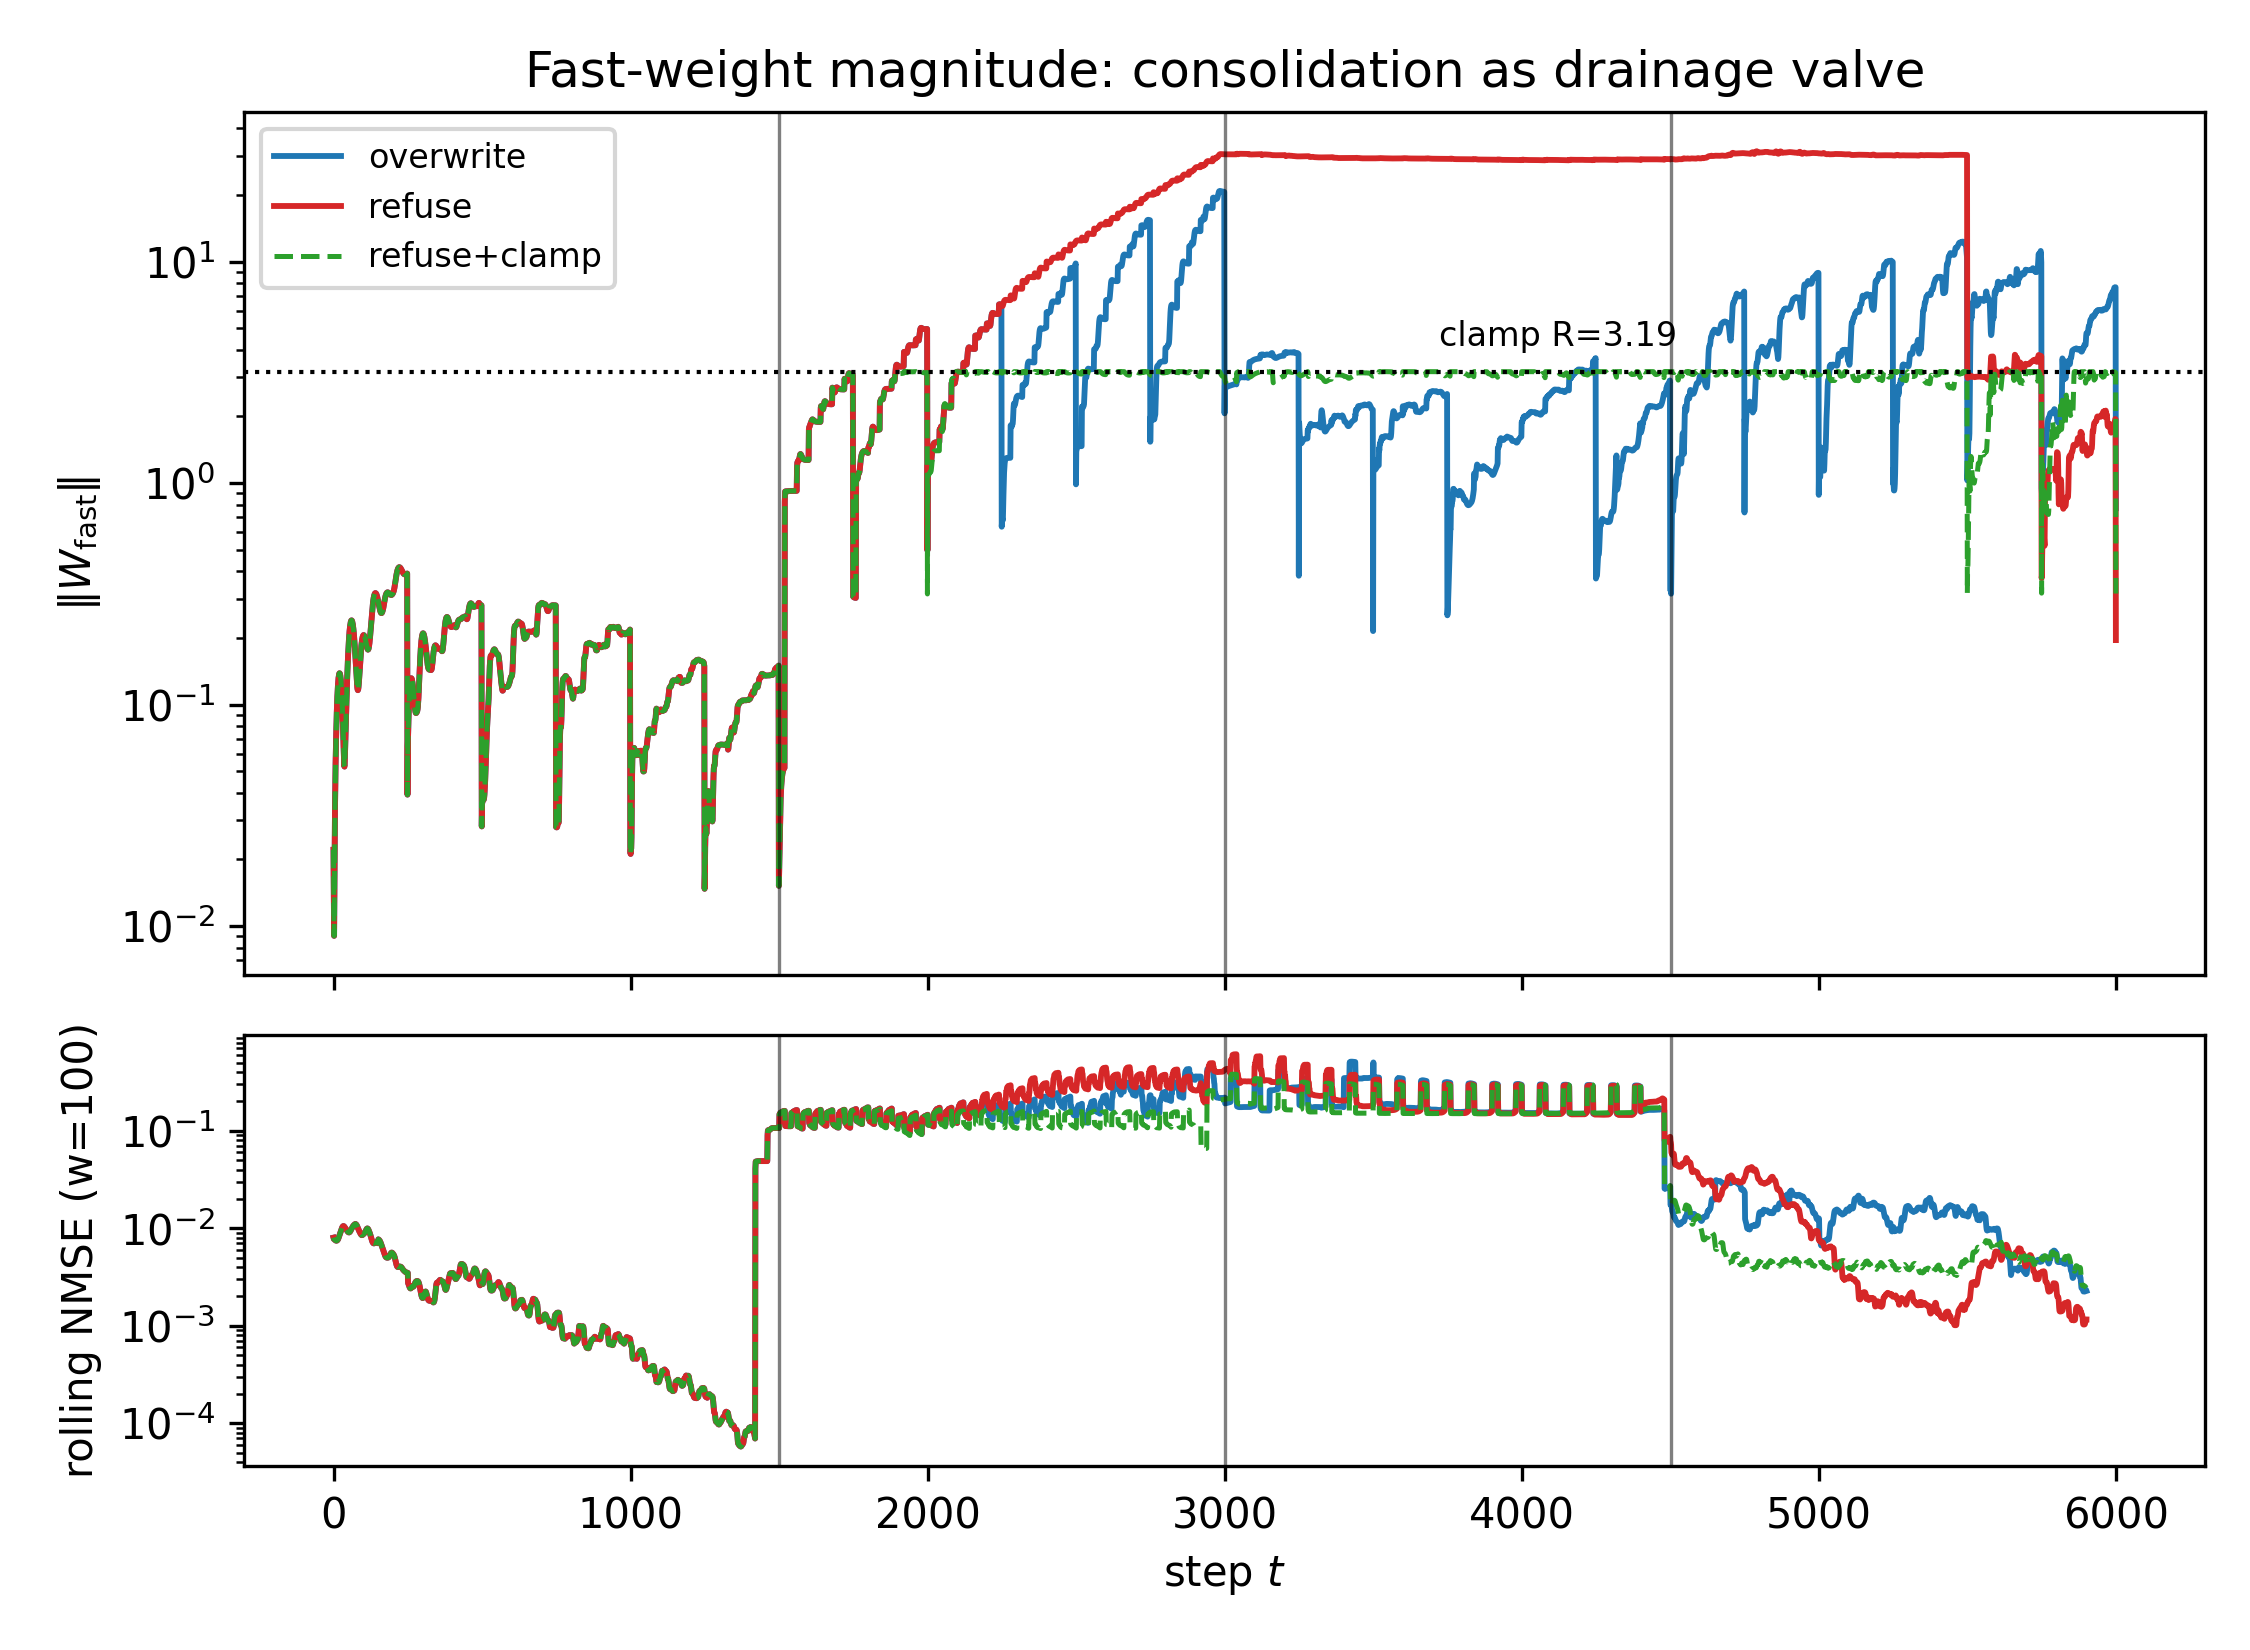
\includegraphics[width=\columnwidth]{fig6_valve.png}
\caption{Consolidation as drainage valve (4-regime overload, seed 0). Top: $\|W_{\mathrm{fast}}\|$ --- refuse lets it wind to $\sim 35$, overwrite drains to $\sim 0.3$, the clamp caps it at $R{=}3.18$. Bottom: rolling NMSE --- refuse loses the onset but wins the tail (it never pays the $\gamma$-decay cost).}
\label{fig:valve}
\end{figure}

\begin{table}[t]
\centering\small
\caption{Per-step operation and memory envelope of the full system.}
\label{tab:table7}
\begin{tabular}{lcc}
\toprule
Component & Ops/step & Memory (float64) \\
\midrule
ESN: $W_{\mathrm{res}}x + W_{\mathrm{in}}u$ + tanh & $\approx$1.1k MAC & $W_{\mathrm{res}}$ 8 kB + $W_{\mathrm{in}}$ 1 kB \\
Spline map & $O(DK)\approx10^{3}$ & $\phi$ buffer 8 kB \\
Block-RLS & $O(DK^{2})\approx10^{4}$ & $P$ 78 kB + $W_{\mathrm{fast}}$ 8 kB \\
Ctx.\ memory & $O(SF)\approx3\cdot10^{3}$ & $W_{\mathrm{slow}}$ 24 kB \\
\textbf{Total} & $\approx$130 \textmu s (Python, full update path) & \textbf{$\approx$0.13 MB} \\
\bottomrule
\end{tabular}
\end{table}

Memory figures are float64 as implemented; float32 halves them. All
learning is local and online; the prototype is pure NumPy, so the
FLOP envelope --- not the wall-clock --- is the hardware-relevant figure for
FPGA/photonic mapping discussed as future work.

\section{Discussion}\label{discussion}

\textbf{A unifying view: gated vs.~ungated channels.} Every result in this
paper reduces to one decomposition,
\[
\hat y_t=\underbrace{\phi_t^\top W_{\mathrm{fast}}}_{\text{ungated —
cannot be suppressed}}+\ \beta\,\phi_t^\top\!\underbrace{\Big(\textstyle\sum_i w_i
W_{\mathrm{slow}}^{(i)}\Big)}_{\text{gated — suppressible}},
\]
and one operation --- consolidation --- whose real function is not
``storage'' but \emph{migrating regime-specific information from the
ungated channel into the gated one}, where the gate can later select
or suppress it. On regime return the gate can zero a slot holding
stale content; it cannot zero whatever square-regime knowledge still
resides in \(W_{\mathrm{fast}}\). This single principle explains the
whole ablation: naive memory consolidates but offers only one slot ---
no selective suppression is possible, so it performs like the
baseline; self-masking (v0) freezes the gate, again collapsing to one
effective channel; v1/v2 migrate correctly but consult a fallible
occupancy oracle; and the \emph{refuse} saturation policy stops the
migration entirely, stranding the current regime's information in the
ungated channel where it interferes at the next transition (Sec.
4.6). The same valve also predicts the mechanism's cost: periodic
\(\gamma\)-decay that drains \(W_{\mathrm{fast}}\) necessarily slows its
final convergence --- the \ctxEndPenalty\(\times\) end-of-phase penalty is not an unrelated
flaw but the price of drainage. Three conditions are jointly
necessary in our ablations: \textbf{\(\ge 2\) separable slots, a correct gate,
and regular drainage} --- remove any one and the system degenerates to
a single channel.

\textbf{Generalizable lessons.} The ablation yields six findings that
extend beyond this architecture. (i) \emph{Unconditional consolidation
relocates forgetting} --- any dual-rate system that copies fast weights
into slow storage on a timer will store the most recent regime, not
the endangered one. (ii) \emph{Self-masking is intrinsic to shared
residuals}: whenever a fast learner is shared across gated
components, its compensation makes the active component look better
than it is; matching scores must exclude the shared predictor. This
applies equally to mixture-of-experts credit assignment and to our
slots. (iii) \emph{Poisoned memory is worse than empty memory} ---
anti-correlated writes produce errors exceeding the empty-slot floor,
so argmin targeting is not safe without a match threshold.
(iv) \emph{Write protection is only as good as its occupancy oracle}:
with an unreliable emptiness proxy (weight norms), protected wrong
targets preserved contamination --- 3/10 seeds regressed --- while the
count rule improved on the norm rule in 10/10 seeds; the proxy, not
the gate, was the bottleneck. (v) \emph{Benefit is proportional
to forgetting cost}: where relearning is cheap or regimes
indistinguishable, the mechanism contributes nothing and costs
nothing --- a graceful degradation we argue should be a design
requirement for continual learners. (vi) \emph{The ungated channel is
the hidden failure locus of fast/slow architectures}: whenever an
always-active component coexists with gateable ones, regime-specific
energy accumulates where it cannot be suppressed --- our refuse
condition stored perfect memory that stayed unreachable beneath
\(\|W_{\mathrm{fast}}\|{\approx}35\) (Sec. 4.6). Two remedies exist:
migrate the content into the gated channel (lossless transfer) or
bound the accumulation (lossy cap, which we show destroys end-phase
accuracy). The structure is not specific to reservoirs --- shared
experts in mixture-of-experts, frozen bases with adapters, and any
residual-coupled modular system expose the same locus.

\textbf{Limitations.} First, the EMA-based matching has an unavoidable
blind spot: after a regime change the fast-error EMA
(\(\alpha_{\mathrm{fast}}{=}0.1\), timescale \(\sim 10\) steps) recovers long
before the slot-error EMA (\(\alpha_{\mathrm{ema}}{=}0.01\), \(\sim 100\)
steps) re-qualifies the correct slot, so contaminating reinforcement
writes slip through --- observed at \(t{=}1750\) in seed 0, where an
early square-adapted \(W_{\mathrm{fast}}\) was written into the sine
slot (bounded: F3 onset still 0.073 on that seed). Second, bootstrap
writes at uniform gates produce bounded
prediction jumps (max 1.49 instantaneous change) --- acceptable in
simulation, but a latency cost at deployment. Third, end-of-phase
accuracy is \ctxEndPenalty\(\times\) worse under retention (\ctxEnd{} vs \blockEnd) --- the
predicted price of regular fast-channel drainage rather than an
unrelated defect; a matched-norm cap is far costlier still (\clampEnd,
Table~\ref{tab:table6}), which is why the design drains by transfer. Fourth, results use a single
hyperparameter set (\(\tau{=}0.5\), \(\eta{=}2\), \(S{=}3\)); a sensitivity sweep is
deferred work. Fifth, the consolidation threshold
conflates \emph{novelty} with \emph{unpredictability}: a single hard regime whose
slow-only error never falls below \(\tau\,\widehat{m_2}\) is perpetually
classified as new context, fragmenting writes across slots (observed as
the 1\(\leftrightarrow 2\) round-robin in the square phase). Consequently the effective
capacity is the number of \emph{allocations}, not regimes --- saturation is
reached before \(S\) distinct regimes. The predicted overload failure
was tested (Sec. 4.6): protection degrades \emph{gracefully} under
count-weighted overwrite (×3--4 retained) but collapses under write
refusal, which starves the \(\gamma\)-decay valve and lets
\(W_{\mathrm{fast}}\) wind up on the unprotected regime. Sixth, the input standardization (stream mean/variance used for
\(u_t\) and the target variance \(\sigma_0\)) is computed from the full
stream as a benchmark constant; deployment would require a fixed
sensor scale or a slow online estimate --- the mechanism itself is
agnostic to this choice. Finally, the task battery covers three
dynamical families; behavior on genuinely stochastic or
high-dimensional streams is untested, and the worst observed single-seed
regression for the final mechanism is 14\% (NARMA test), while the
intermediate norm-proxy variant degraded single seeds by up to 20\%.

\textbf{Future work.} The remaining onset error is attributable to gate
transition latency and residual fast-weight interference; gating the
fast contribution by gate confidence is the natural next step. The
valve analysis suggests a direct improvement: making the
ungated-channel budget an explicit design knob (a norm cap on
\(W_{\mathrm{fast}}\), which alone recovered 0.073\(\to0.019\) under
refuse) could permit a larger \(\gamma\) and thus reduce the
end-of-phase penalty the drainage currently costs.
Dynamic slot allocation (opening slots on context mismatch rather
than fixing S) and comparison with SNN/STDP and hyperdimensional
baselines are planned. On the hardware side, the O(DK²) envelope and
locality of all updates map naturally onto FPGA or analog
crossbar/photonic implementations --- a claim we keep deliberately at
the architectural level pending a system-level energy study.
Finally, preliminary transfer tests on frozen GPT-2 embeddings in a
domain-return classification protocol expose the same mechanism under
a stricter constraint: the gate's slot-error time constant
(\(\alpha_{\mathrm{ema}}\)) must be far shorter than the
regime-transition window to avoid onset poisoning from a stale slot,
and the consolidation trigger must be rescaled to the task's error
baseline --- with a fivefold faster gate the same code reduced
return-onset error from 0.30 to 0.23 on 768-d features.

\section{Conclusion}\label{conclusion}

We have presented a backpropagation-free contextual memory for
online reservoir prediction whose every component is justified by a
measured failure of a simpler mechanism. On the standard
sine→square→sine regime protocol the system reduces return-onset
NMSE ×4.40 with statistical significance across 10 seeds, while
remaining harmless where there is nothing to protect. The
engineering takeaway is that continual learning in linear readouts
does not require gradients, buffers, or Fisher estimates --- it
requires measuring memory quality correctly (excluding the shared
fast learner), writing only when the context is confirmed, and
choosing the write target by counting rather than weighing. Against
the closest prior art --- competitive multi-head readouts --- the
mechanism still gains \(\times\)\residualRatio{} after we strengthen the competitor with
our own allocation trigger and normalized gate, isolating the
residual advantage in the dual-rate transfer architecture. The
scientific takeaway is twofold: dual-rate consolidation is necessary
but not sufficient --- without context-aware write protection, memory
becomes a delayed copy of the very forgetting it was meant to
prevent; and the \emph{ungated} channel is the hidden failure locus of
fast/slow architectures, accumulating regime energy that must either
be migrated into gated storage or bounded at a measured cost to
convergence.

\section*{References}\label{references-verified}

\begin{itemize}
\tightlist
\item
  J. L. McClelland, B. L. McNaughton, R. C. O'Reilly, ``Why there are
  complementary learning systems in the hippocampus and neocortex,''
  Psychological Review, 1995.
\item
  D. Kumaran, D. Hassabis, J. L. McClelland, ``What learning systems do
  intelligent agents need?,'' Trends in Cognitive Sciences, 2016.
\item
  J. Kirkpatrick et al., ``Overcoming catastrophic forgetting in neural
  networks,'' PNAS, 2017. (EWC)
\item
  F. Zenke, B. Poole, S. Ganguli, ``Continual learning through synaptic
  intelligence,'' ICML, 2017. (SI)
\item
  D. Lopez-Paz, M. Ranzato, ``Gradient episodic memory for continual
  learning,'' NeurIPS, 2017. (GEM)
\item
  D. Rolnick, A. Ahuja, J. Schwarz, T. Lillicrap, G. Wayne, ``Experience
  replay for continual learning,'' NeurIPS, 2019.
\item
  H. Jaeger, ``The `echo state' approach to analysing and training
  recurrent neural networks,'' GMD Report 148, 2001.
\item
  M. Lukoševičius, H. Jaeger, ``Reservoir computing approaches to
  recurrent neural network training,'' Computer Science Review, 2009.
\item
  D. Sussillo, L. F. Abbott, ``Generating coherent patterns of activity
  from chaotic neural networks,'' Neuron, 2009. (FORCE)
\item
  K. J. Åström, B. Wittenmark, Adaptive Control, 2nd ed., 1995.
\item
  R. A. Jacobs, M. I. Jordan, S. J. Nowlan, G. E. Hinton, ``Adaptive
  mixtures of local experts,'' Neural Computation, 1991.
\item
  N. Shazeer et al., ``Outrageously large neural networks: The
  sparsely-gated mixture-of-experts layer,'' ICLR, 2017.
\item
  Z. Liu et al., ``KAN: Kolmogorov--Arnold Networks,'' arXiv:2404.19756,

  \begin{enumerate}
  \def\labelenumi{\arabic{enumi}.}
  \setcounter{enumi}{2023}
  \tightlist
  \item
  \end{enumerate}
\item
  A. Cossu, D. Bacciu, A. Carta, C. Gallicchio, V. Lomonaco,
  ``Continual learning with echo state networks,''
  arXiv:2105.07674, 2021.
\item
  L. Bereska and E. Gavves, ``Continual learning of dynamical systems
  with competitive federated reservoir computing,'' PMLR 199:335--350,

  \begin{enumerate}
  \def\labelenumi{\arabic{enumi}.}
  \setcounter{enumi}{2021}
  \tightlist
  \item
    Code: github.com/leonardbereska/multiheadreservoir.
  \end{enumerate}
\item
  D. M. Wolpert, M. Kawato, ``Multiple paired forward and inverse models
  for motor control,'' Neural Networks, 1998. (MOSAIC)
\item
  J. Schwarz et al., ``Progress \& Compress: A scalable framework for
  continual learning,'' ICML, 2018.
\item
  J. Gama, I. Žliobaitė, A. Bifet, M. Pechenizkiy, A. Bouchachia, ``A
  survey on concept drift adaptation,'' ACM Computing Surveys, 2014.
\item
  K. Vandoorne et al., ``Experimental demonstration of reservoir
  computing on a silicon photonics chip,'' Nature Communications 5,
  3541, 2014.
\item
  R. Elwell, R. Polikar, ``Incremental learning of concept drift in
  nonstationary environments,'' IEEE Trans. Neural Networks 22(10),
  1517--1531, 2011. (Learn++.NSE)
\end{itemize}

\appendix
\section{Per-seed Results}\label{appendix-a-per-seed-results}

F3-onset NMSE (250-step window) per seed on the main
sine→square→sine protocol. MH is bit-identical to Block-RLS in 9/10
seeds (its passive protection never engages); seed 6 is the single
exception. CTX v3 (final) improves on the baseline in 10/10 seeds and
on v2 in 10/10 seeds; v2's three regressions against v1 are marked \(^{*}\).

\begin{table}[t]
\centering\small
\caption{Per-seed F3-onset NMSE (250-step window) on the main
protocol. MH is bit-identical to Block-RLS in 9/10 seeds; CTX v3
improves on the baseline in 10/10 and on v2 in 10/10; v2's three
regressions against v1 are marked $^{*}$.}
\label{tab:tableA}
\begin{tabular}{lcccccccc}
\toprule
seed & Block & naive & MH & MH+alloc & v0 & v1 & v2 & v3 (final) \\
\midrule
0 & 0.180 & 0.180 & 0.180 & 0.180 & 0.180 & 0.139 & 0.173$^{*}$ & 0.073 \\
1 & 0.500 & 0.498 & 0.500 & 0.318 & 0.497 & 0.298 & 0.265 & 0.125 \\
2 & 0.312 & 0.312 & 0.312 & 0.317 & 0.378 & 0.367 & 0.246 & 0.113 \\
3 & 0.247 & 0.245 & 0.247 & 0.247 & 0.245 & 0.128 & 0.105 & 0.098 \\
4 & 0.666 & 0.658 & 0.666 & 0.679 & 0.658 & 0.180 & 0.120 & 0.073 \\
5 & 0.260 & 0.260 & 0.260 & 0.260 & 0.262 & 0.244 & 0.296$^{*}$ & 0.113 \\
6 & 0.913 & 0.905 & 0.546 & 0.458 & 0.830 & 0.186 & 0.171 & 0.081 \\
7 & 0.463 & 0.457 & 0.463 & 0.461 & 0.455 & 0.199 & 0.202$^{*}$ & 0.127 \\
8 & 0.660 & 0.655 & 0.660 & 0.364 & 0.637 & 0.153 & 0.115 & 0.094 \\
9 & 0.385 & 0.384 & 0.385 & 0.408 & 0.403 & 0.145 & 0.135 & 0.067 \\
\midrule
mean & 0.459 & 0.455 & 0.422 & 0.369 & 0.455 & 0.204 & 0.183 & \textbf{0.096} \\
\bottomrule
\end{tabular}
\end{table}

Strengthened-competitor runs (Table~\ref{tab:table3b}), same seeds ---
\texttt{MH+soft} is the non-orthogonality check of Sec. 4.3:

\begin{table}[h]
\centering\small
\caption{Strengthened-competitor per-seed runs; MH+soft is the
non-orthogonality check of Sec. 4.3.}
\label{tab:tableB}
\begin{tabular}{lcc}
\toprule
seed & MH+soft & MH+alloc+soft \\
\midrule
0 & 0.175 & 0.175 \\
1 & 0.314 & 0.185 \\
2 & 0.219 & 0.203 \\
3 & 0.241 & 0.241 \\
4 & 0.476 & 0.487 \\
5 & 0.250 & 0.250 \\
6 & 0.317 & 0.297 \\
7 & 0.362 & 0.365 \\
8 & 0.386 & 0.172 \\
9 & 0.287 & 0.304 \\
\midrule
mean & 0.303 & 0.268 \\
\bottomrule
\end{tabular}
\end{table}

\section*{Code and Data Availability}\label{code-and-data-availability}

All results are produced by deterministic, seed-resolved scripts
using \texttt{np.random.default\_rng(seed)} --- seeds 0--9 (main) and 0--4
(generalization):

\begin{itemize}
\tightlist
\item
  \url{benchmark_block_rls.py} --- RLS characterization (Table~\ref{tab:table1})
\item
  \url{continual_protocol.py} --- stream builder + main protocol
\item
  \url{different_tasks.py} --- cross-family generalization (Table~\ref{tab:table4})
\item
  \url{make_figures.py} --- Figs. 3--5 and \url{metrics.json}/\url{fig_data.npz}
\item
  \url{saturation_test.py}, \url{valve_test.py} --- Table~\ref{tab:table5}, Fig.~\ref{fig:valve}, \url{saturation_data.npz}, \url{valve_data.npz}
\item
  \url{clamp_control.py} --- main-protocol drainage control (Table~\ref{tab:table6}, \url{clamp_control.json})
\item
  \url{fig2_windup.py}, \url{fig1_architecture.py} --- Figs. 1--2
\end{itemize}

Aggregated metrics are emitted to \url{metrics.json}; per-seed arrays to
\url{fig_data.npz}, \url{saturation_data.npz}, \url{valve_data.npz}, and
\url{clamp_control.json}, from which every table and figure in this
paper is generated. Code and data are publicly available at
\url{https://github.com/GhostPookie/contextual-consolidation-rc};
hardware and software versions are listed in Sec. 4.1.

\end{document}
